Dans les disques isothermes, la migration de Type I est gouvernée par le couple différentiel de Lindblad et le couple de corotation, qui induisent généralement
une migration vers l'intérieur \citep{goldreich1980disk, ward1986density, tanaka2002three}. Dans les disques radiatifs, un terme supplémentaire du couple de corotation provenant d'un gradient d'entropie peut contrebalancer le couple
différentiel de Lindblad sous certaines conditions et ainsi inverser le sens de migration (vers l'extérieur)
\citep{paardekooper2006halting, kley2008migration}. Il est donc possible d'avoir dans un disque des zones où la migration
s'arrête. Ces zones sont appelées zone de convergence \citep[CZs;][]{lyra2010orbital,
paardekooper2011torque, hellary2012global}. 

\bigskip

À la zone de convergence, le couple de corotation (positif) compense exactement le couple différentiel de Lindblad (négatif).
Ainsi, à la zone de convergence, une planète ne migre pas.

De plus, autour de la zone de convergence, la migration tend à ramener les embryons vers la zone de couple nul s'ils s'en
éloignent. La zone de convergence est donc une position stable dans le disque vers laquelle les embryons se rassemblent.

Il peut exister de même des zones de couples nuls qui ne sont pas des zones de convergence quand, en s'éloignant légèrement, la
migration tend à les éloigner davantage. Ces zones sont alors instables.

Les zones de convergences pourraient ainsi concentrer les embryons planétaires et être le lieu de formation de planètes (ou
cœurs) massives \citep{lyra2010orbital, horn2012orbital}. 

\bigskip

Je vais montrer dans les paragraphes qui suivent que la migration est extrêmement sensible aux paramètres du disque.

\cite{kretke2012importance} ont étudié l'influence des paramètres du disque sur la migration. Cependant, s'ils ont inclus des
effets fins sur le bord interne et la migration, la dépendance de l'opacité en fonction de la température et de la densité est
approximée par différentes lois de puissance. Nous montrerons que l'opacité est un paramètre sensible du modèle et qu'il est
important de la modéliser le plus finement possible. 

\cite{bitsch2013influence} ont étudié en particulier l'effet de la viscosité $\nu$ et l'indice adiabatique $\gamma$ sur la
migration dans le disque, au travers de simulations 3D. 

Afin d'étudier séparément l'effet des paramètres du disque, j'ai choisi un disque de référence, décrit
\refsec{sec:migrations-maps}. Dans cette partie je présente les cartes de migration et comment les interpréter. En particulier
je présente la carte de migration du disque de référence \reffig{fig:fiducial_migration_map}. Pour chaque paramètre, je vais
donc conserver les valeurs du disque de référence, et faire varier le paramètre en question autour de la valeur de référence. Sauf
mention contraire, un seul paramètre est donc modifié à la fois, seuls les paramètres qui changent sont précisés, les autres
sont regroupés \reftab{tab:fiducial_parameters}.

\section{Disque de référence}\label{sec:migrations-maps}\label{sec:reference_disk}

\begin{figure}[htbp]
\centering
\subfloat[Couple Adimensionné]{\label{fig:fiducial_adim}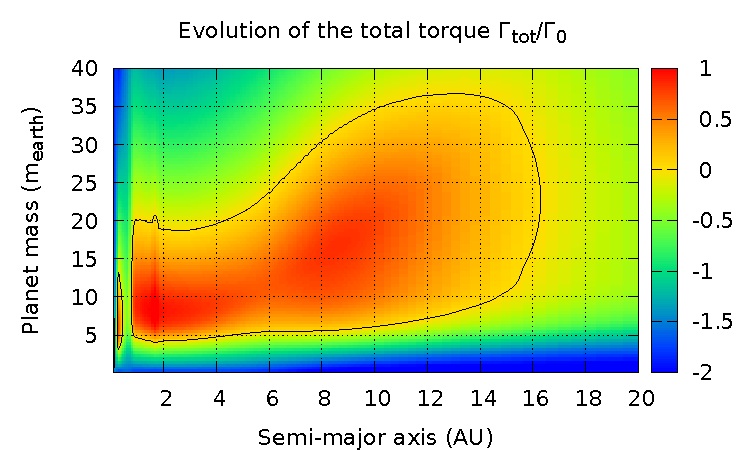
\includegraphics[width=0.49\textwidth]{figure/migration_map/fiducial.pdf}}\hfill
\subfloat[Couple Réel]{\label{fig:fiducial_units}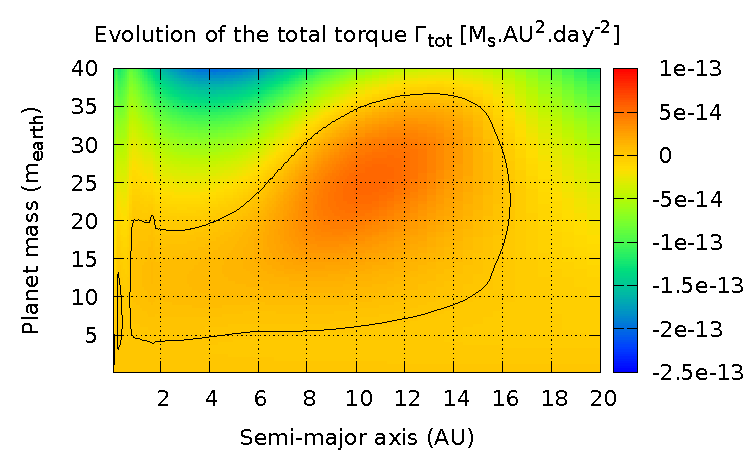
\includegraphics[width=0.49\textwidth]{%
figure/migration_map/fiducial_units.pdf}}

\caption[Carte de migration pour le disque de référence.]{Carte de migration pour le disque de référence. Cette carte montre le
sens de migration d'une planète en fonction de sa
position (abscisse) et de sa masse (ordonnée). La 3\ieme coordonnée est le couple total exercé par le disque sur la planète,
exprimé en unité de $\Gamma_0 = \left(\frac{q}{h}\right)^2\Sigma_p {r_p}^4 {\Omega_p}^2$ pour la carte de gauche, et en \unit{M_\odot UA^2/jour^2} pour la carte de droite. Quand le couple est positif (resp.
négatif), la migration est vers l'extérieur (resp. intérieur). La ligne noire représente la zone de couple nul, où la planète ne
migre plus. Le détail des paramètres du disque de référence est donné \reftab{tab:fiducial_parameters}.
}\label{fig:fiducial_migration_map}
\end{figure}

Dans cette partie, nous allons présenter notre disque de référence et comment ses paramètres vont influencer la migration des
planètes. Ce disque de référence servira aussi de comparaison quand nous étudierons les effets des paramètres du disque.

Ce disque est obtenu à l'aide de la table d'opacité d'\cite{hure2000transition}. Le profil de température est
calculé en tenant compte de l'irradiation, avec des paramètres solaires pour la température et le rayon de l'étoile ($T_\star =
5700\unit{K}$ ; $R_\star = 4.65\cdot 10^{-3}\unit{UA}$). L'albédo du disque est pris égal à $0.5$. La viscosité est calculée à
partir d'une prescription alpha \citep{shakura1973black}. On considère un disque dont les bords internes et externes sont
respectivement à $0.1$ et $100\unit{UA}$. Les autres paramètres du disques sont récapitulés \reftab{tab:fiducial_parameters}. 

\begin{table}[htbp]
\centering
\begin{tabular}{|c|c|c|c|}
\hline
$b/h = 0.4$ & $\gamma = 7/5$ & $\mu = 2.35$ & $\alpha = 5\cdot 10^{-3}$ \\\hline
\multicolumn{2}{|c|}{Inner edge : $0.1\unit{UA}$} & \multicolumn{2}{c|}{Outer edge : $100\unit{UA}$}\\\hline
\multicolumn{2}{|c|}{$\Sigma(R) = 300 \cdot R^{-1/2}\unit{g/cm^2}$}& \multicolumn{2}{c|}{$M_\text{tot} = 0.14\unit{M_\odot}$}\\\hline
$T_\star = 5700\unit{K}$ & $R_\star = 4.65\cdot 10^{-3}\unit{UA}$ & \multicolumn{2}{c|}{Disk albedo : $0.5$}\\\hline
\end{tabular}
\caption[Paramètres physiques du disque de référence.]{Paramètres physiques du disque de référence. Les opacités sont calculées
à partir de la table d'opacité de
\cite{hure2000transition}. La viscosité est calculée en suivant la prescription alpha de
\cite{shakura1973black}.}\label{tab:fiducial_parameters}
\end{table}

La longueur de lissage $b/h$ est prise assez faible afin de ne pas sous-estimer le couple de corotation, qui est la partie la plus importante du couple dans notre cas car c'est celle qui permet d'inverser le sens de migration. En faisant cela, on sur-estime le couple de Lindblad, pour lequel une longueur de lissage de $b/h=0.75$ est conseillée \citep{masset2002coorbital}.
En considérant que le gaz du disque est un gaz parfait diatomique, l'indice adiabatique vaut alors $\gamma=7/5$.
La valeur de $\alpha$ correspond à une valeur typique observée. De plus, elle tient compte du fait que la viscosité diminue avec l'âge du disque et que nous considérons une époque où le disque a déjà évolué, puisque nous prenons des embryons relativement massifs (au minimum $0.1\mearth$). De même, le profil de densité de surface $\Sigma(R) = 300 \cdot R^{-1/2}\unit{g/cm^2}$ ne correspond pas à un disque très massif car on considère que le disque est déjà évolué. 

Afin d'étudier la migration dans les disques, il est pratique de 
regarder une \og carte de migration\fg, comme \reffig
{fig:fiducial_migration_map}. Cette carte permet de voir rapidement 
les parties intéressantes et de prédire l'évolution d'une planète à 
partir des position et masse initiales. Le couple adimensionné 
\reffig{fig:fiducial_adim} sera préférentiellement utilisé quand 
nous représenterons une carte de migration ensuite, car plus intuitif 
à lire. La carte \reffig{fig:fiducial_units} montre que le couple 
total a des dépendances complexes au travers de $\Gamma_0$. Il 
dépend notamment de la masse de la planète, du rapport d'aspect et 
de la densité locale du disque. \reffig{fig:fiducial_migration_map} montre la carte de migration du disque de référence que nous utiliserons de manière
récurrente ici. 

\begin{figure}[htbp]
\centering
\subfloat[Lindblad torque]{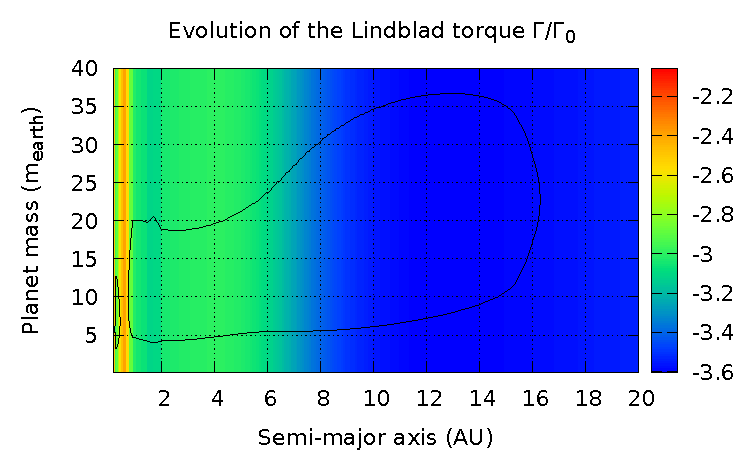
\includegraphics[width=0.49\textwidth]{figure/migration_map/details/lindblad_torque.pdf}}\hfill
\subfloat[Entropy-related horseshoe drag]{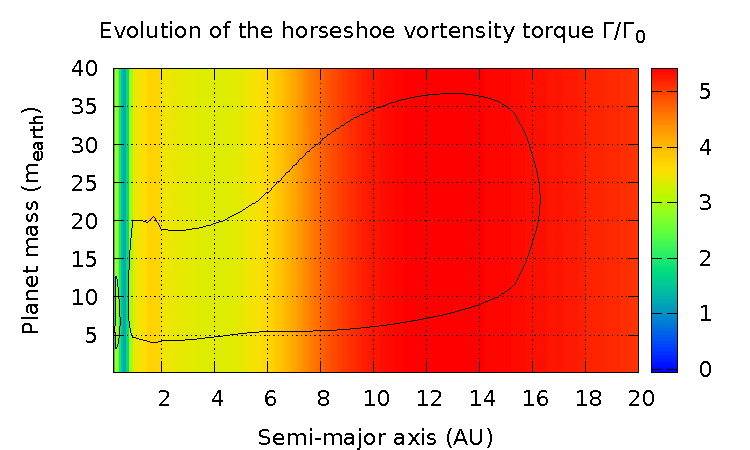
\includegraphics[width=0.49\textwidth]{%
figure/migration_map/details/ent_hs_torque.pdf}}

\caption[Carte des couples de Linblad et corotation.]{Évolution des deux couples les plus importants vis à vis de la carte de
migration, le couple de Lindblad et la partie
non saturée du couple de corotation liée au gradient d'entropie. En effet, ces deux couples sont quantitativement plus grands que
tous les autres. Ici, seule la partie non-saturée du couple de corotation est représentée.}\label{fig:details_maps}
\end{figure}

Sur \reffig{fig:details_maps} sont représentés les deux couples les plus importants en terme d'amplitude. D'une part le couple négatif dominant, le
couple de Lindblad $\Gamma_L$, et d'autre part le couple positif dominant, la partie du couple de corotation non saturée liée au gradient d'entropie
$\Gamma_\text{ent,hs}$. Ici, c'est bien la partie non saturée qui est représentée (fully unsaturated horseshoe drag en anglais). On ne tient pas
compte de la diffusion. On constate alors que sans tenir compte de la diffusion, les couples sont totalement indépendants de la
masse. La transition que l'on constate dans les deux cartes, entre $6-8\unit{UA}$ correspond à la transition disque
actif/passif. L'irradiation est le processus de chauffage principal à partir de $5\unit{UA}$ comme illustré par
\reffig{fig:viscous_vs_irradiation}.

\begin{figure}[htbp]
\centering
\subfloat[$t_\text{rad}/t_\text{U-turn}$]{\label{fig:linear_rad}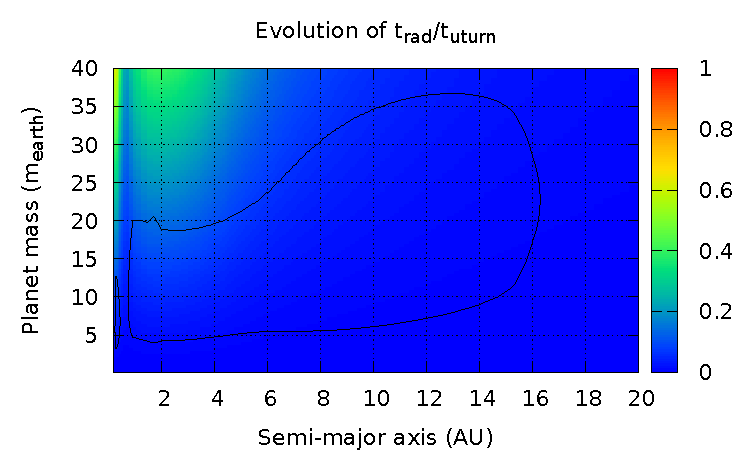
\includegraphics[width=0.49\textwidth]{%
figure/timescales/linear_rad.pdf}}\hfill
\subfloat[Saturation : $(t_\text{lib}/2)/t_\text{visc}$]{\label{fig:sat_visc}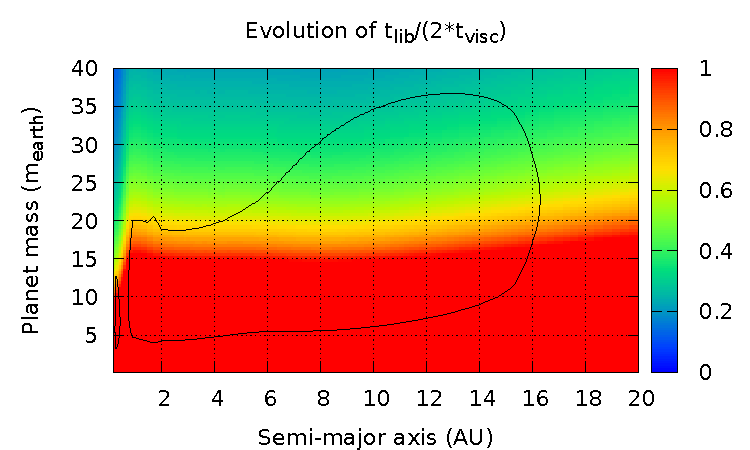
\includegraphics[width=0.49\textwidth]{%
figure/timescales/sat_visc.pdf}}

\caption[Cartes des temps de diffusions dans le disque.]{Comparaison des différents temps caractéristiques influençant le couple
de corotation. Ces inéquations sont détaillées
dans \refsec{sec:couple-corotation}. Dans le cas présent, le temps de diffusion radiative est toujours plus court que le temps
de diffusion visqueuse, $t_\text{rad}<t_\text{visc}$. Ainsi il ne reste plus que les deux inégalités représentées
ici. La saturation est ainsi gouvernée par le temps de diffusion visqueux $t_\text{visc}$. La transition couple non-saturé/couple linéaire est elle déterminée par le temps de diffusion radiatif $t_\text{rad}$.}\label{fig:timescales_maps}
\end{figure}

\reffig{fig:timescales_maps} représente l'effet de la diffusion sur la carte de migration. Dans le cas d'un disque purement actif, on s'attend à ce que $t_\text{rad}=t_\text{visc}$ car $\nu\propto\xi$. Ici, à cause de l'irradiation, nous avons $t_\text{rad}<t_\text{visc}$, la saturation est alors gouvernée par le temps de diffusion visqueux $t_\text{visc}$ et la transition couple non-saturé/couple linéaire est déterminée par le temps de diffusion radiatif $t_\text{rad}$. Ainsi, seules deux inégalités sont ici nécessaires pour étudier le couple de corotation :
\begin{align}
t_\text{U-turn} < t_\text{diff} < \frac{t_\text{lib}}{2}\\\nonumber
t_\text{U-turn} < t_\text{rad} < t_\text{visc} < \frac{t_\text{lib}}{2}
\end{align}

Sur \reffig{fig:timescales_maps} on remarque que les parties active et passive du disque sont distinctes. En dessous de $4\unit{UA}$, la partie supérieure de la carte de migration s'explique par la saturation du couple de corotation. La ligne de couple nul suit en effet l'équation $(t_\text{lib}/2) = t_\text{visc}$ \reffig{fig:sat_visc}.

La partie inférieure quant à elle, s'explique par la transition entre le couple non saturé et le couple linéaire pour le couple de corotation. La ligne de couple nul suit en effet l'équation $t_\text{U-turn} = t_\text{rad}$ \reffig{fig:linear_rad}. Le couple de corotation devient linéaire quand le temps de diffusion radiatif est trop court pour permettre à un gradient de s'installer dans la zone fer-à-cheval.

\begin{figure}[htbp]
\centering
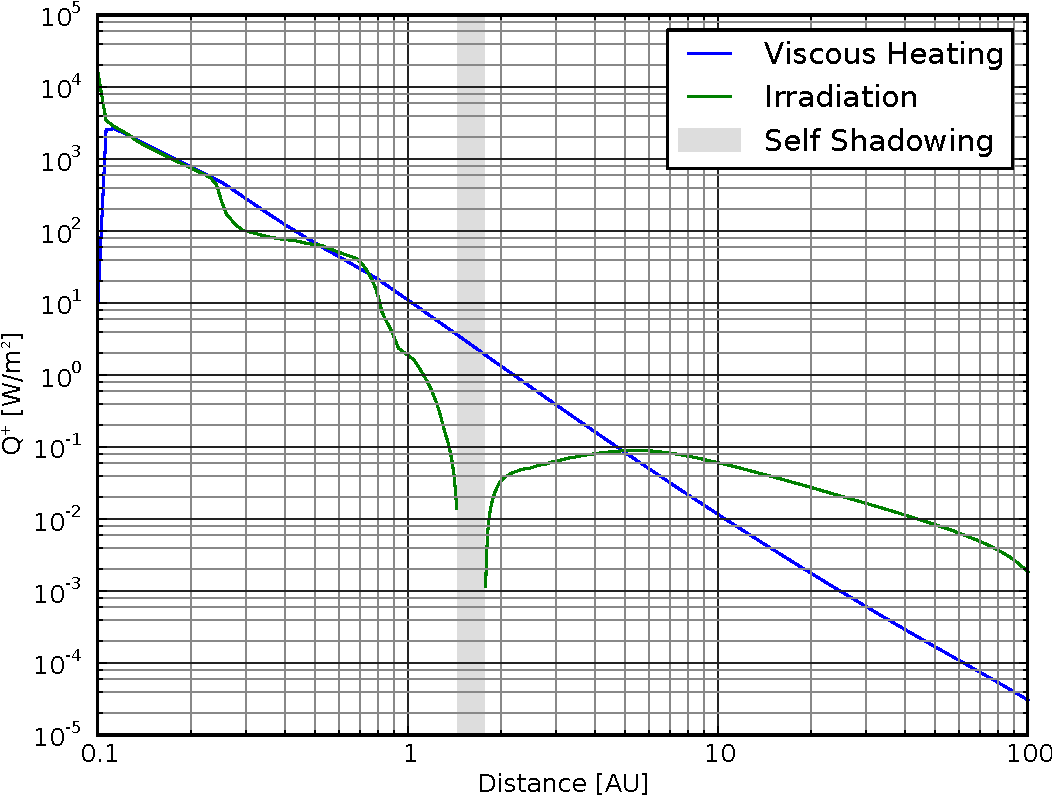
\includegraphics[width=0.75\textwidth]{figure/migration_map/viscous_vs_irradiation.pdf}

\caption[Amplitude du chauffage visqueux et de l'irradiation dans le disque.]{Amplitude des termes sources dans l'équation
d'énergie liés au chauffage visqueux et à l'irradiation. Dans les parties internes, c'est le
chauffage visqueux qui domine. Dans les parties externes c'est l'irradiation. À $5\unit{UA}$ les deux contributions sont
égales. La partie grisée correspond à la zone où l'irradiation est forcée à 0 car l'angle d'interception des rayons solaires est négatif (l'échelle de hauteur diminue). Ce n'est donc pas à proprement parler un \og Self-Shadowing\fg qui concerne une zone beaucoup plus étendue.}\label{fig:viscous_vs_irradiation}
\end{figure}

À partir de $5\unit{UA}$, l'irradiation domine le bilan énergétique \reffig{fig:viscous_vs_irradiation} et une simple comparaison des temps de diffusion ne permet plus d'expliquer simplement l'allure de la carte de migration. Ce n'est plus seulement les temps de diffusion qui permettent de trouver la zone de couple nul dans le disque, mais les valeurs des couples eux mêmes. Au delà de $4\unit{UA}$, sans tenir compte de la saturation les couples augmentent différemment. En effet, au delà de $4\unit{UA}$, le profil de température est dominé par l'irradiation et l'indice du gradient de température diminue avec la distance à partir de $d=1$ à $4\unit{UA}$ jusqu'à $d=0.5$ à $40\unit{UA}$. Les couples de Lindblad et de corotation n'ayant pas les mêmes dépendances vis à vis du gradient de température, l'écart entre les couples change.

La fermeture des parties externes de la carte de migration s'explique donc par l'action conjointe de la diffusion radiative et visqueuse. Pour les masses
faibles, en dessous de $15-20\mearth$, la migration vers l'intérieur est due au fait que $t_\text{U-turn} > t_\text{rad}$, c'est
alors la valeur linéaire du couple de corotation qui prévaut. Pour les masses plus importantes, le couple de corotation sature
car $(t_\text{lib}/2) < t_\text{visc}$. 

\bigskip

Avant $1\unit{UA}$, deux régions de couples positifs sont séparées par une région peu étendue où la migration est dirigée vers l'intérieur. C'est une transition d'opacité à $1\unit{UA}$ qui
en est la cause, et qui change brusquement les couples de migration \reffig{fig:details_maps}. Ce
brusque changement d'opacité et de température est la raison de la séparation de la zone de couple positif en deux. 

Nous avons alors deux zones de couple nul dont l'origine physique et les propriétés sont quelques peu différentes. 

\section{Différents types de zone de convergence}\label{sec:CZ-types}\index{zone de convergence}
À partir de ces cartes de migration nous pouvons étudier l'évolution des différentes zones de couple nul en fonction de la
distance. Ces zones sont représentées par une ligne noire. Nous pouvons dégager deux types particulier de zones de convergence. 

Le premier type de zone de convergence est ce que nous appellerons une \textbf{zone de convergence indépendante de la masse}. C'est une
zone qui se trouve plutôt dans les parties internes du disque et est généralement créée par une transition d'opacité. Cette ligne de couple nul dépend très peu de la masse de la
planète car une transition d'opacité induit de brusques changements de température. Les couples varient ainsi fortement sur une
distance très courte. Cette zone de convergence a deux caractéristiques importantes : 
\begin{enumerate}
\item La position de la zone de convergence ne dépend pas ou peu de la masse de planète
\item La variation du couple de migration autour de la zone de convergence est très forte
\end{enumerate}

Nous pouvons appeler le deuxième type \textbf{zone de convergence dépendant de la masse}. En effet, dans les parties externes, le
couple varie plus doucement en fonction de la distance. L'influence de la masse est donc plus marquée dans la position de la zone
de couple nul. Ce type de zone de convergence a deux caractéristiques importantes : 
\begin{enumerate}
\item La position de la zone de convergence dépend de la masse de la planète. 
\item Le couple de migration varie doucement en fonction de la distance à la zone de convergence
\end{enumerate}

\begin{figure}[htbp]
\centering
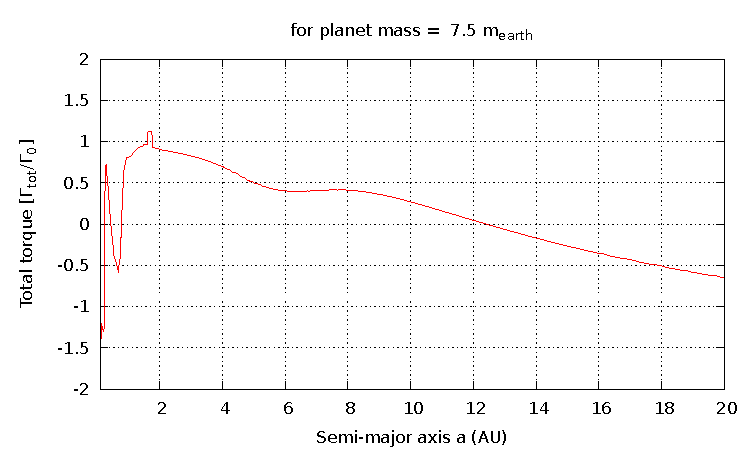
\includegraphics[width=0.75\linewidth]{figure/total_torque_fixed_m.pdf}
\caption{Évolution du couple total exercé par
le disque sur une planète de $7.5\mearth$. }\label{fig:total_torque_fixed_m}
\end{figure}

\reffig{fig:total_torque_fixed_m} illustre les deux zones de convergences. La première près de $1\unit{UA}$, siège d'une
variation brutale du couple de migration, et la deuxième (dont la position dépend de la masse de la planète) où la variation du
couple de migration est continue. 

Dans la suite, nous utiliserons parfois des zones de convergences artificielles afin de simplifier les effets, et d'étudier
plus facilement un phénomène particulier. Dans le cas d'une transition d'opacité, nous avons modélisé les zones de convergence
indépendantes de la masse par une fonction tangente hyperbolique dont le zéro se situe à la zone de convergence, et où le couple de
migration (positif ou négatif) sature très loin de la zone de convergence \refsec{sec:tanh_indep}. Pour modéliser une zone de
convergence indépendante de la masse où le couple varie peu autour de la zone de convergence, nous avons utilisé une variation
linéaire du couple de migration \refsec{sec:linear_indep}.

Les zones de convergence dépendantes de la masse peuvent être approximées par une variation linéaire de la position de la zone
de couple nul en fonction de la masse. Le couple de migration varie quant à lui linéairement en fonction de la distance
\refsec{sec:mass_dependant}. 

\bigskip

Il existe malgré tout un point commun aux zones de convergence, quelque soit leur type. Une planète doit être suffisamment massive pour migrer vers la zone de convergence. En dessous d'une masse critique, les embryons migrent vers l'intérieur. La zone de convergence ne peut donc rassembler les embryons qu'à partir d'une certaine masse, de l'ordre de plusieurs masses terrestres. Un autre processus, différent de la migration convergente d'embryons vers une zone de convergence doit donc permettre la formation de ces embryons planétaires massifs pour que ceux-ci se rassemblent à la zone de convergence.

En fonction de la distance, nous pouvons définir des masses critiques extrémales au delà desquelles la migration vers
l'extérieur est impossible en raison du temps de diffusion qui est soit trop grand (saturation) soit trop petit (couple
linéaire) pour que le couple de corotation soit suffisamment important.

La zone ne convergence ne peut exister que pour une certaine gamme de masses de planète. Au delà de ces limites, la planète trop ou trop peu massive migrera vers l'intérieur.

\section{Effet de l'irradiation}\index{irradiation}
En choisissant ou non d'inclure l'irradiation dans l'équation de l'énergie permettant de calculer le profil de température, on
change de manière importante la carte de migration \citep{bitsch2013stellar}. 

\begin{figure}[htbp]
\centering
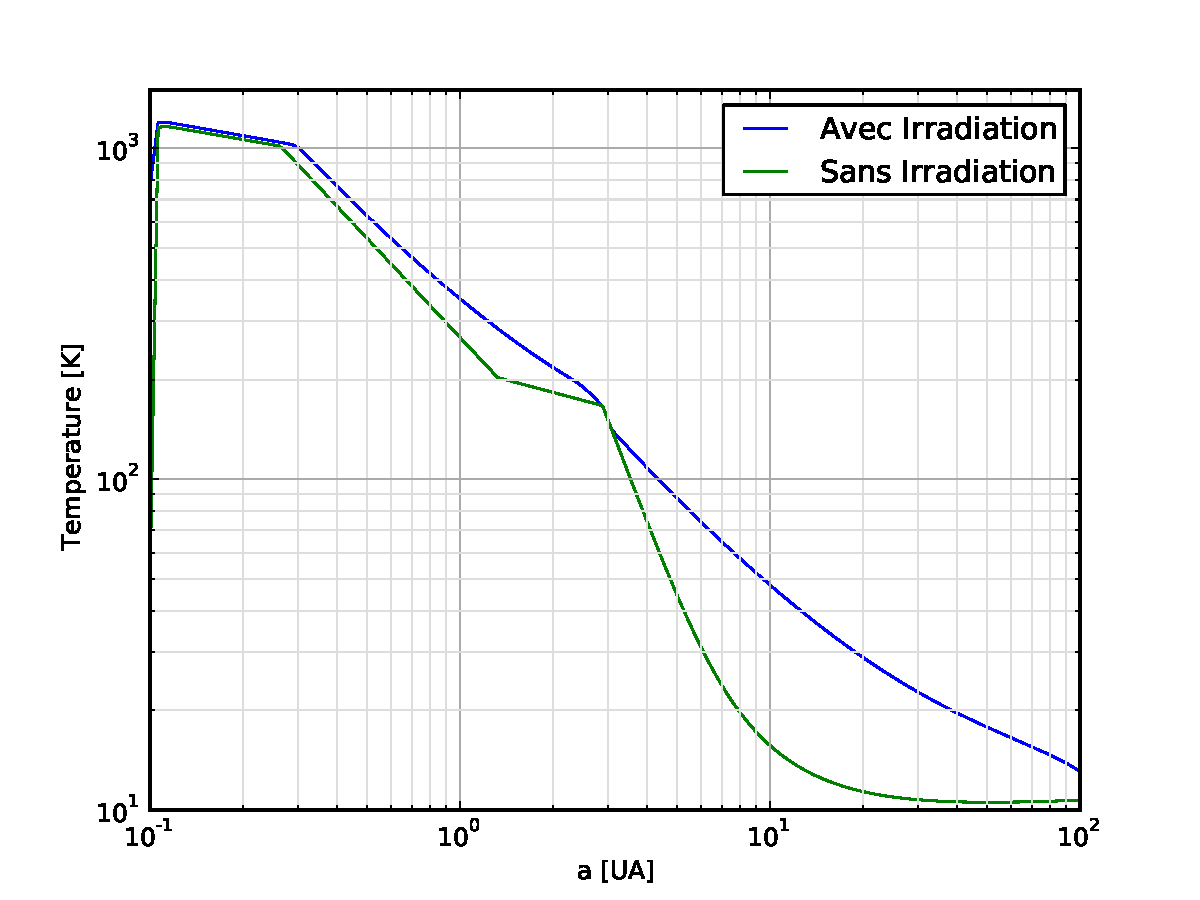
\includegraphics[width=0.6\linewidth]{figure/migration_map/temperature_with_irradiation.pdf}
\caption[Profil de température avec ou sans irradiation.]{Profil de température avec ou sans irradiation.
\refdisk}\label{fig:temp_profile_irradiation}
\end{figure}


Afin de visualiser l'effet de l'irradiation, nous avons utilisé les lois d'opacités de \cite{bell1994FU}. En effet,
le principal effet de l'irradiation est de lisser le profil de température. Sans irradiation, une discontinuité dans le régime d'opacité comme celles de \cite{bell1994FU} se répercute directement sur le profil de température \reffig{fig:temp_profile_irradiation}.
On voit donc apparaître des zone de convergences dues à des transitions d'opacités mais qui sont déformées par
l'irradiation comme on peut le constater sur \reffig{fig:irradiation}.

\begin{figure}[htbp]
\centering
\subfloat[Avec irradiation]{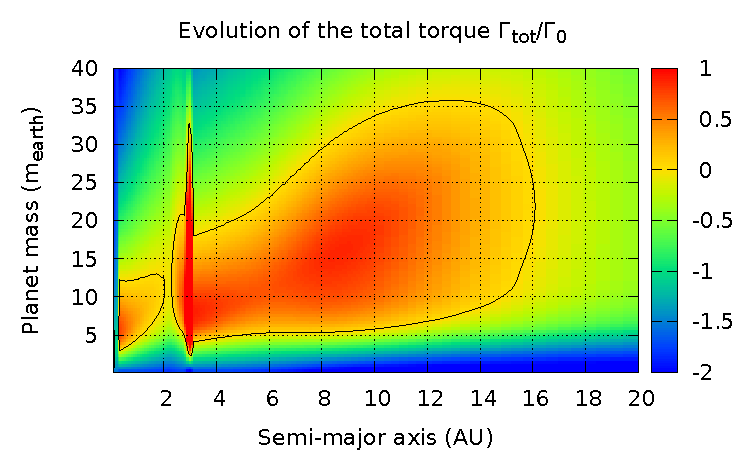
\includegraphics[width=0.49\textwidth]{figure/migration_map/bell_irr.pdf}}\hfill
\subfloat[Sans irradiation]{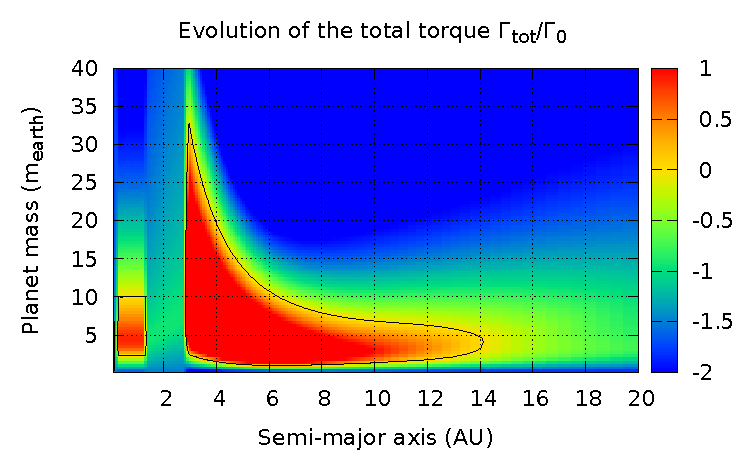
\includegraphics[width=0.49\textwidth]{%
figure/migration_map/bell_noirr.pdf}}

\caption[Carte de migration avec ou sans irradiation.]{Influence de l'irradiation sur la carte de migration à travers le profil
de température. Afin de visualiser plus
facilement les effets, l'opacité de \cite{bell1994FU} a été utilisée. \refdisk}\label{fig:irradiation}
\end{figure}

Ainsi, sans irradiation, les deux transitions d'opacités à $1.3$ et $2.9\unit{UA}$ induisent un changement brutal de la pente
du profil de température, ce qui a pour effet de changer le sens de migration (de positif à négatif, puis l'inverse).

Dans les parties externes, l'irradiation a pour effet de diminuer la pente du profil de température qui tend vers un profil en
$R^{-\sfrac37}$ quand le disque est purement passif.


\subsection{Effet de l'ombre du disque sur lui même.}\label{sec:shadow}\index{self-shadowing}
Tout au long de ma thèse, j'ai considéré un modèle d'irradiation dans lequel la gestion des ombres restait sommaire. En effet, la seule ombre que je considérais était l'ombre directe. C'est à dire les régions du disque pour lesquelles l'échelle de hauteur décroit avec la distance. Ces zones où l'angle d'interception des rayons de l'étoile était négatif étaient détectées et l'irradiation était forcée à zéro. Nous appellerons ce modèle le \textbf{modèle direct}. C'est un modèle qui découle naturellement de la modélisation du disque. En effet, pour calculer le profil de température, on doit calculer la température point par point en partant du bord externe pour que le calcul de la température converge. Nous n'avons donc pas accès à l'ombre réelle du disque lors du calcul de l'irradiation. L'ombre est simplement la zone où l'angle entre les rayons de l'étoile et la surface du disque est nul.

Ici nous cherchons à comparer ce modèle avec deux modèles plus complexes où l'ombre du disque est gérée de manière plus cohérente. 

Dans ces nouveaux modèles, on calcule une première fois le profil de température du disque et on stocke la valeur de l'irradiation en chaque point du disque. Ensuite, on détecte les ombres du disque en cherchant les maxima locaux du profil d'échelle de hauteur. Pour chaque maximum local, on cherche l'ombre qu'il projette sur le disque et dans cette ombre là, l'irradiation est forcée à 0. Dans les derniers 10\% de l'étendue de l'ombre, on lisse linéairement l'irradiation en considérant que 10\% avant la fin de l'ombre, l'irradiation est égale à $0 * F_\text{irr}$ (où $F_\text{irr}$ est le chauffage d'irradiation local) et à la toute fin de l'ombre, l'irradiation vaut $1 * F_\text{irr}$. Ainsi, à la position $R_b + 0.95 * l_s$ (où $R_b$ est le rayon de la bosse du disque considérée et $l_s$ est la longueur de l'ombre qu'il projette), l'irradiation vaut la moitié de l'irradiation calculée précédemment $0.5 * F_\text{irr}$. 

J'ai testé deux cas, un cas où l'étoile est considérée ponctuelle, que nous nommerons \textbf{modèle ponctuel}, et un cas où on prend en compte le rayon de l'étoile que nous appellerons le \textbf{modèle étendu}. Dans ce dernier cas, on néglige totalement le fait qu'en sortant de l'ombre, on ne voit quasiment pas l'étoile. Dans tous les modèles, l'irradiation considère que l'étoile n'est pas ponctuelle, c'est simplement pour le calcul des ombres a posteriori que l'on considèrera soit une étoile ponctuelle soit de rayon $R_\star$.

\reffig{fig:shadow_temp_profile} montre l'évolution du profil de température en fonction des différents modèles de l'ombre du disque. Le profil de température du \textbf{modèle direct} est simplement celui du disque de référence. L'ombre est simplement constituée des zones où l'angle de réception des rayons de l'étoile est nul. Dans ce cas, la zone d'ombre est située entre $1.46$ et $1.75\unit{UA}$.

\begin{figure}[htbp]
\centering
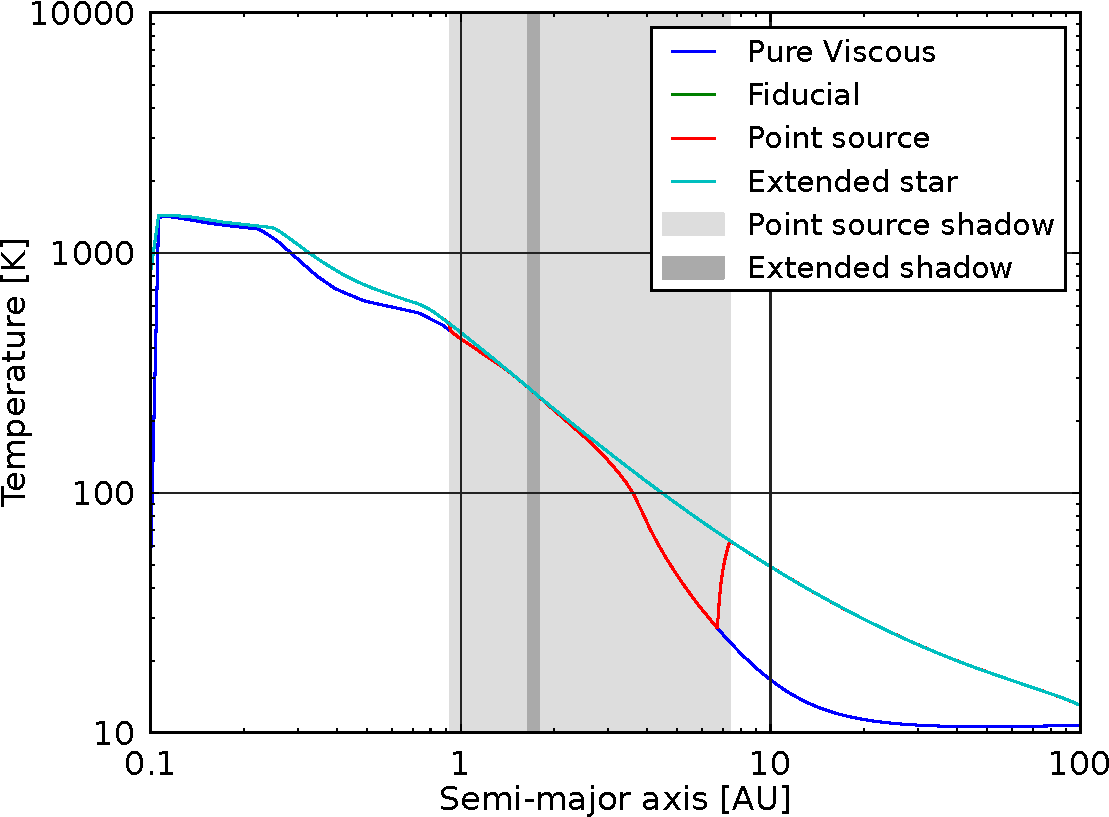
\includegraphics[width=0.49\textwidth]{figure/shadow/fiducial_temperature_profile.pdf}

\caption[Influence de l'ombre sur le profil de température]{Profils de température pour différents modèles où l'ombre du disque
sur lui-même est calculée différemment. Les profils des modèles \textbf{direct} et \textbf{étendu} sont confondus.
\refdisk}\label{fig:shadow_temp_profile}
\end{figure}

Ensuite, le \textbf{modèle ponctuel} considère l'étoile centrale comme ponctuelle, et cherche \textit{a posteriori} les ombres du disques, avant de recalculer une nouvelle fois le profil de température. Le profil de température du disque de référence dans lequel on ne tient pas compte de l'irradiation (chauffage visqueux uniquement) est représenté, afin de pouvoir comparer. Dans la zone d'ombre ainsi calculée, le profil de température est équivalent à un profil purement visqueux, sans tenir compte de l'irradiation de l'étoile. En effet, dans cette région là, l'irradiation est forcée à 0. 

Maintenant, on considère que l'étoile possède un rayon $R_\star=R_\odot$ (\textbf{modèle étendu}), l'ombre qui s'étendait auparavant de $0.93$ à $7.35\unit{UA}$ dans le \textbf{modèle ponctuel} n'est plus que de $1.65$ à $1.78\unit{UA}$. L'ombre commence plus loin, car les rayons de l'étoile centrale partent de plus haut. Ils ne partent plus de $z=0$ mais de $z=0.0046\unit{UA}$. De même, la surface du disque sort beaucoup plus rapidement de l'ombre pour les mêmes raisons. En conséquence, le \textbf{modèle étendu} possède exactement le même profil que le \textbf{modèle direct}. L'ombre est dans ce cas située dans une partie totalement dominée par le chauffage visqueux et l'irradiation n'a aucune incidence sur la température du disque. 

\begin{figure}[htbp]
\centering
\subfloat[Modèle
ponctuel]{\label{fig:extended_shadow_map}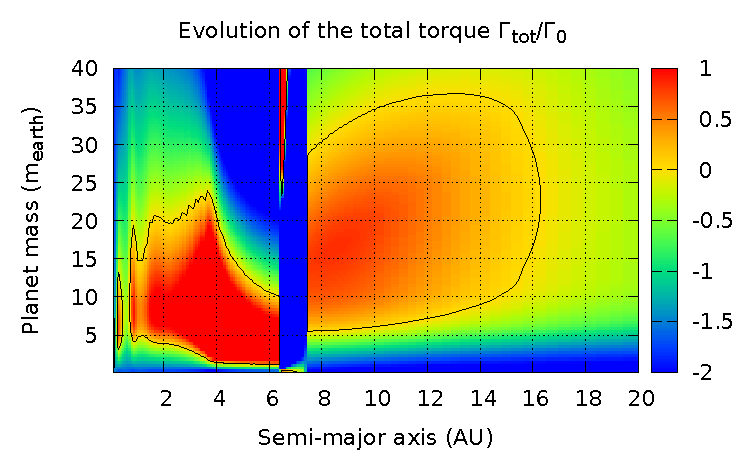
\includegraphics[width=0.49\textwidth]{figure/shadow/fiducial_shadow.pdf}}\hfill
\subfloat[Modèle étendu]{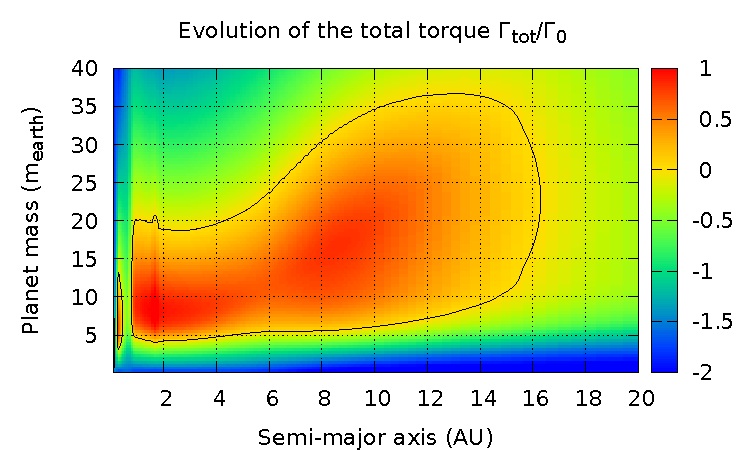
\includegraphics[width=0.49\textwidth]{%
figure/shadow/fiducial_r_star_shadow.pdf}}

\caption[Influence de l'ombre sur la carte de migration.]{Influence de la modélisation de l'ombre sur la carte de migration. 
\refdisk}\label{fig:map_shadow_effect}
\end{figure}

Les profils de températures avec les deux nouveaux modèles testés, à savoir les modèles \textbf{ponctuel} et \textbf{étendu},
nous donnent les cartes de migration \reffig{fig:map_shadow_effect}. Dans le cadre du \textbf{modèle ponctuel}, la région
d'ombre change la carte de migration. Dans l'ombre, et juste avant d'en sortir, la carte de migration est équivalente à un
disque purement actif, sans irradiation. En dehors de l'ombre, la carte de migration ne change pas. Mais à la fin de l'ombre,
près de $6\unit{UA}$, alors que le chauffage par irradiation remonte brusquement dans la région où l'ombre n'est plus
complète, une zone de transition apparait. Dans cette zone, la température monte brusquement, et le profil s'inverse. Pour les
très grandes ($m>25\mearth$) et très petite ($m<1\mearth$) masses, une zone de migration vers l'extérieur apparait, permettant
de maintenir ces planètes dans le disque, alors que les masses intermédiaires ne peuvent pas migrer vers l'extérieur dans cette
région de transition \reffig{fig:extended_shadow_map}. 

Dans le cas du \textbf{modèle étendu}, la carte de migration ne change pas par rapport au disque de référence. Dans ce modèle, l'ombre n'est pas suffisamment étendue pour atteindre les parties passives du disque, où l'irradiation est importante. Ainsi, désactiver l'irradiation ne change pas le profil de température et la migration n'est ainsi pas affectée. 

Le modèle le plus abouti pour le calcul de l'ombre est le \textbf{modèle étendu} qui recalcule l'ombre a posteriori mais prend en compte la non ponctualité de l'étoile. 

Pour que le calcul de l'ombre du disque ait une importance sur la carte de migration, il faut que la bosse du disque soit suffisamment importante pour qu'une partie de l'ombre soit projetée dans la partie passive du disque, là où l'irradiation est importante. \reffig{fig:shadow-example} montre un exemple d'un disque où la modélisation de l'ombre a une importance. Dans ce disque, nous avons toujours les propriétés du disque de référence, à ceci près que le profil de densité est maintenant $\Sigma(R) = 1700 * R^{-1.5}\unit{g/cm^2}$. 

\begin{figure}[htbp]
\centering
\subfloat[Modèle direct]{\label{fig:label1}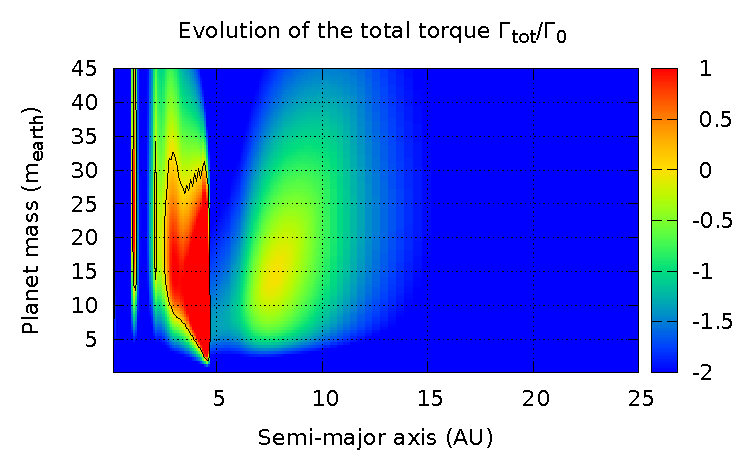
\includegraphics[width=0.49\textwidth]{figure/shadow/example_with_direct_shadow.pdf}}\hfill
\subfloat[Modèle étendu]{\label{fig:label2}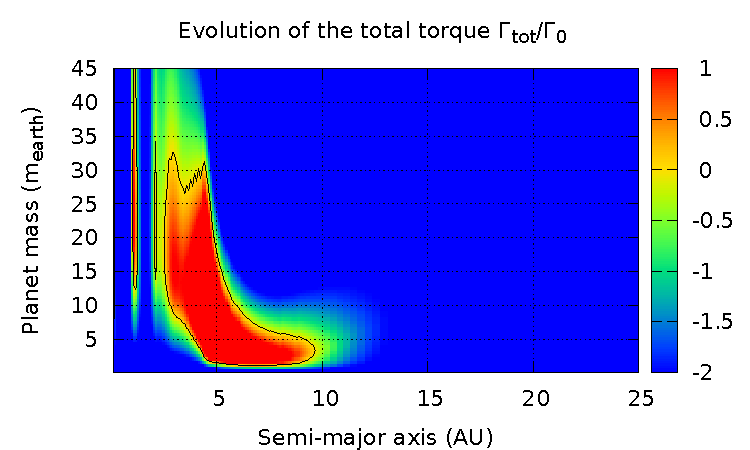
\includegraphics[width=0.49\textwidth]{figure/shadow/example_with_shadow.pdf}}
\caption[Influence de l'ombre sur la carte de migration d'un disque massif.]{Effet des modèles pour l'ombre du disque sur la
carte de migration dans un cas où la densité de surface vaut $\Sigma(R) = 1700 * R^{-1.5}\unit{g/cm^2}$.
\refdisk}\label{fig:shadow-example}
\end{figure}

Dans ce cas, la température extrêmement élevée au bord interne cause l'apparition d'une bosse très importante au bord interne du disque qui masque totalement l'étoile dans le cas où le calcul de l'ombre du disque se fait a posteriori. Les deux profils de température et les ombres correspondantes sont représentés \reffig{fig:example_shadow_temp_profile}. 

\begin{figure}[htbp]
\centering
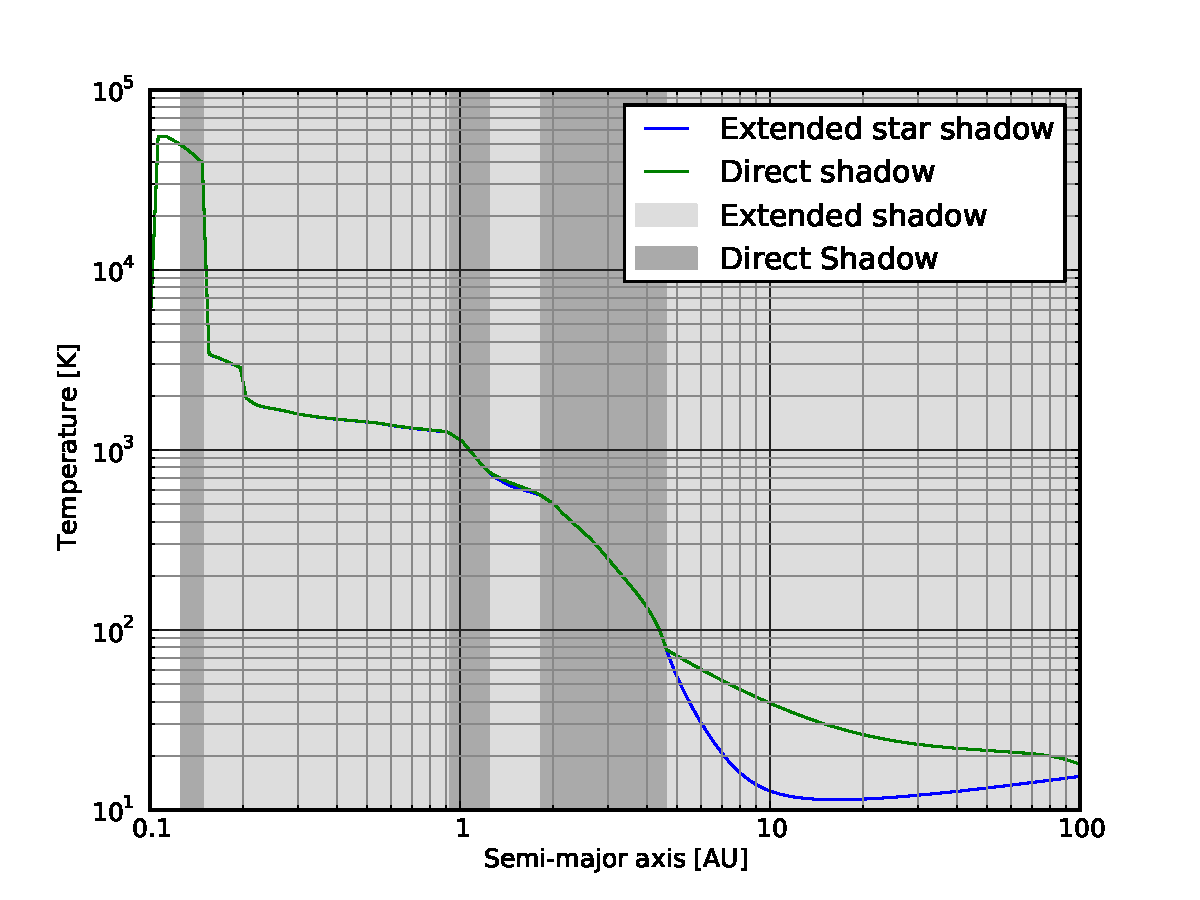
\includegraphics[width=0.65\linewidth]{figure/shadow/example_shadow_temp_profile.pdf}
\caption[Influence de l'ombre sur le profil de température d'un disque massif.]{Profil de température et ombre du disque dans le
cas du modèle direct ou étendu pour la modélisation de l'ombre. La densité de surface vaut $\Sigma(R) = 1700 *
R^{-1.5}\unit{g/cm^2}$. \refdisk}\label{fig:example_shadow_temp_profile}
\end{figure}

Malgré tout, le \textbf{modèle étendu} ne prend pas en compte le fait qu'au delà de cette zone d'ombre, il y a toute une zone où l'irradiation de l'étoile est partielle, dû au fait qu'une partie de l'étoile est masquée par le disque. Il ne prend pas non plus en compte l'auto-irradiation, c'est à dire le fait que des parties du disques peuvent en illuminer d'autres, compte tenu du fait qu'on a le profil d'échelle de hauteur qui se creuse à cet endroit là. Cet effet sera d'autant plus marqué que la température du disque est importante et que la bosse du disque est grande. 

De plus, les cas où ce nouveau modèle pour l'ombre du disque a un effet important sont des cas limites. En effet, dans l'exemple présenté ici \reffig{fig:shadow-example}, la température au bord interne dépasse $50 000\unit{K}$. Dans des disques beaucoup plus classiques, avec des températures inférieures à $10 000\unit{K}$ au bord interne, nous avons vu que le modèle classique pour l'ombre du disque marchait bien, car l'ombre se trouvait dans la partie active du disque, là où l'irradiation joue un rôle mineur sur le profil de température.

\subsection{Effet des propriétés de l'étoile}
Pour le modèle de référence, les propriétés de l'étoile sont celles du Soleil, même rayon même température. Mais les propriétés des étoiles au moment de la formation planétaire ne sont pas celles d'une étoile évoluée comme le Soleil. Elles ont tendance à être moins chaudes, et plus grosses que le Soleil. À partir de \cite[Table 2]{hartigan1995disk}, \reffig{fig:TTauri_sample} représente 42 étoiles T Tauri dans un diagramme avec leur rayon en abscisse et leur température en ordonnée. 

\begin{figure}[htbp]
\centering
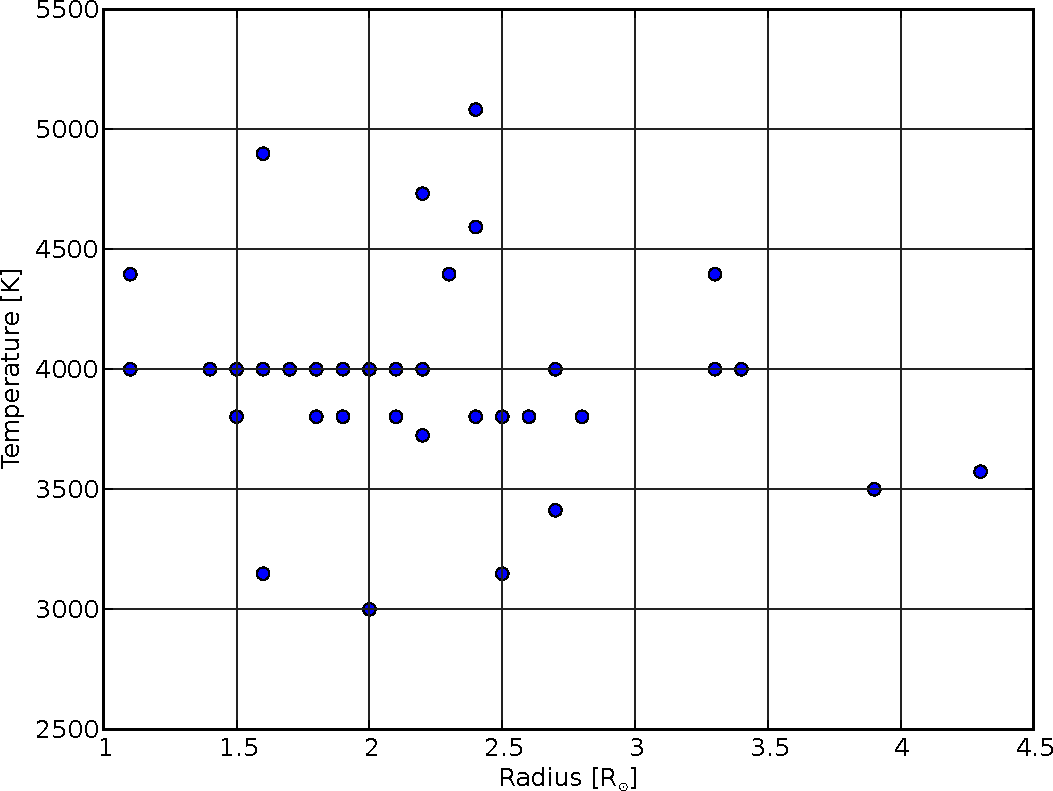
\includegraphics[width=0.5\linewidth]{figure/TTauri_sample.pdf}
\caption[Propriétés d'un échantillon d'étoiles T Tauri détectées.]{Représentation d'un échantillon d'étoiles TTauri
\citep{hartigan1995disk}. }\label{fig:TTauri_sample}
\end{figure}

Nous souhaitons voir l'influence des propriétés de l'étoile vis à vis de l'irradiation. Nous allons maintenant faire varier le rayon $R_\star$ et la température $T_\star$ de l'étoile au centre du disque. 

\begin{figure}[htbp]
\centering
\subfloat[$R_\star=1.5\unit{R_\odot}$ ; $T=4000\unit{K}$]{\label{fig:low_TTauri}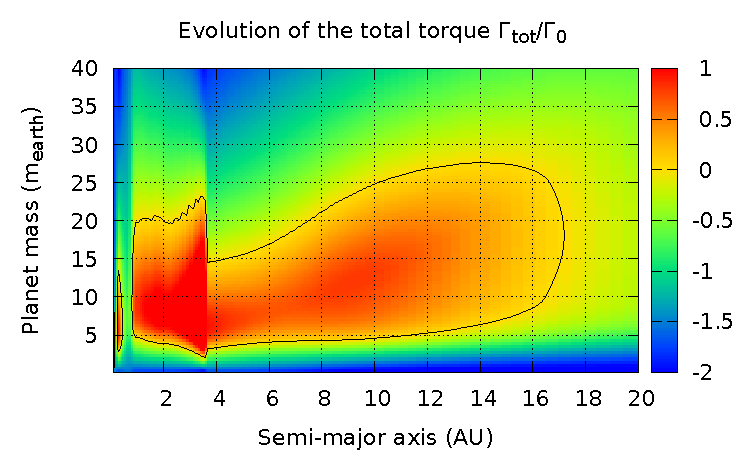
\includegraphics[width=0.49\textwidth]{figure/migration_map/TTauri/R_15_T_4000.pdf}}
\hfill
\subfloat[$R_\star=2.5\unit{R_\odot}$ ; $T=3500\unit{K}$]{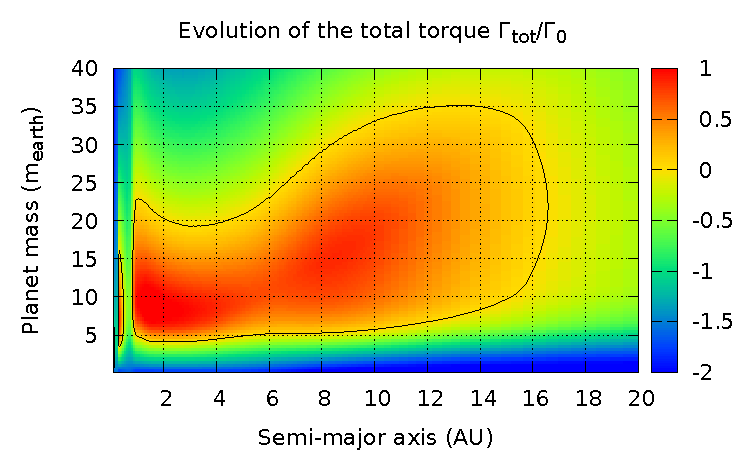
\includegraphics[width=0.49\textwidth]{%
figure/migration_map/TTauri/R_25_T_3500.pdf}}

\subfloat[$R_\star=2.5\unit{R_\odot}$ ; $T=4000\unit{K}$]{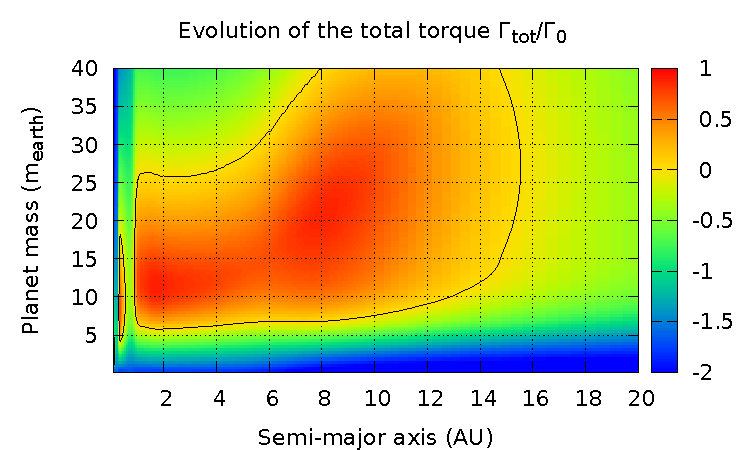
\includegraphics[width=0.49\textwidth]{figure/migration_map/TTauri/R_25_T_4000.pdf}}\hfill
\subfloat[$R_\star=2.5\unit{R_\odot}$ ; $T=4500\unit{K}$]{\label{fig:high_TTauri}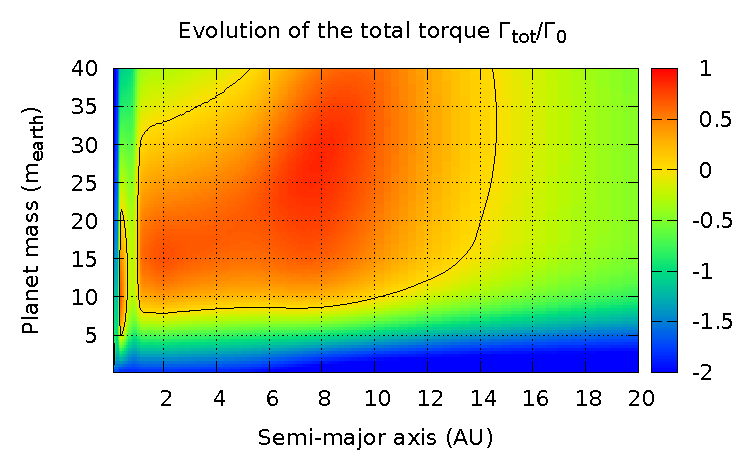
\includegraphics[width=0.49\textwidth]{figure/migration_map/TTauri/R_25_T_4500.pdf}}
\caption[Influence des propriétés de l'étoile centrale sur la carte de migration.]{Influence du rayon $R_\star$ et de la
température $T_\star$ de l'étoile centrale sur la carte de migration au travers de l'irradiation. Les luminosités
correspondantes pour les cartes (a), (b), (c) et (d) sont respectivement $0.5\unit{L_\odot}$, $0.84\unit{L_\odot}$,
$1.43\unit{L_\odot}$ et $2.30\unit{L_\odot}$. \refdisk}\label{fig:map_TTauri}
\end{figure}

À partir des 4 étoiles TTauri typiques que nous avons choisies, nous avons l'effet de la luminosité de l'étoile sur la carte de migration. En effet, il y a une dégénérescence entre le rayon et la température de l'étoile, si on considère une étoile ponctuelle. Les cartes ont été classées de la plus faible à la plus grande luminosité, les luminosités allant de $0.5\unit{L_\odot}$ à $2.30\unit{L_\odot}$. À mesure que l'irradiation de l'étoile augmente, le profil de température augmente au travers du disque de manière quasi uniforme. L'irradiation joue ici sur les masses critiques minimales et maximales au delà desquelles la migration vers l'intérieur est systématique. En particulier, les planètes de $4\mearth$ peuvent migrer vers l'extérieur dans le premier disque \reffig{fig:low_TTauri}, alors qu'il faut qu'elle aient au minimum $8\mearth$ pour pouvoir migrer dans le dernier disque \reffig{fig:high_TTauri} où l'irradiation est la plus forte. 

\bigskip

Nous avons vu dans la partie précédente l'effet de l'ombre du disque. Nous souhaitons maintenant voir ce qu'il en est quand, à
luminosité constante, on varie le rayon et la température de l'étoile \reffig{fig:map_TTauri_radius}. À mesure que le rayon de
l'étoile augmente, les ombres du disque s'amenuisent car les parties supérieures de la sphère stellaire deviennent visibles.
Ainsi, on remarque que la bosse sur la carte de migration disparait à mesure que le rayon de l'étoile augmente. 

\begin{figure}[htbp]
\centering
\subfloat[$R_\star=0.5\unit{R_\odot}$ ; $T=8061\unit{K}$]{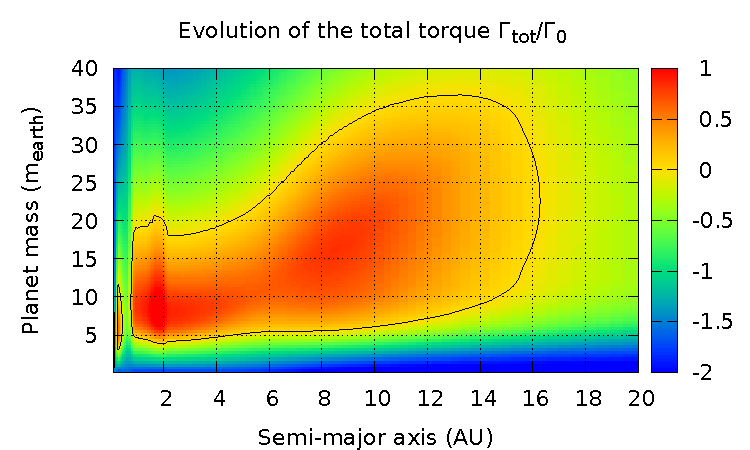
\includegraphics[width=0.49\textwidth]{figure/migration_map/TTauri/R_05_T_8061.pdf}}
\hfill
\subfloat[$R_\star=\unit{R_\odot}$ ; $T=5700\unit{K}$]{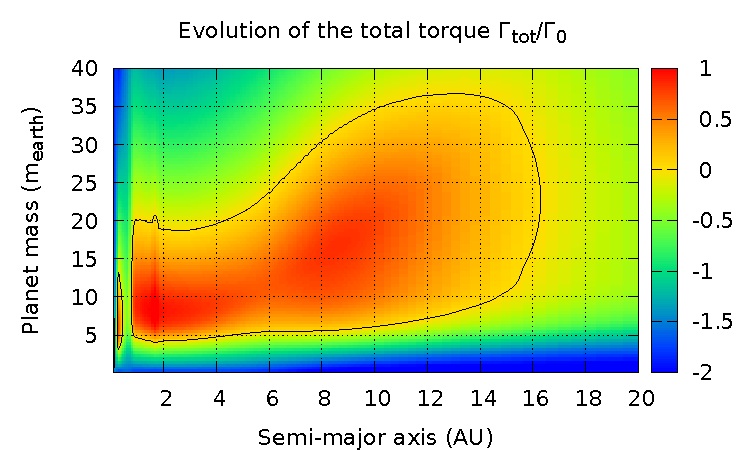
\includegraphics[width=0.49\textwidth]{%
figure/migration_map/TTauri/R_10_T_5700.pdf}}

\subfloat[$R_\star=2\unit{R_\odot}$ ; $T=4031\unit{K}$]{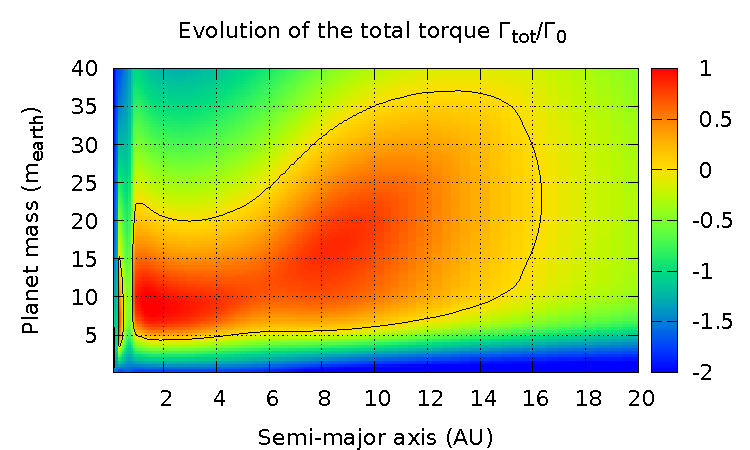
\includegraphics[width=0.49\textwidth]{figure/migration_map/TTauri/R_20_T_4031.pdf}}\hfill
\subfloat[$R_\star=4\unit{R_\odot}$ ; $T=2850\unit{K}$]{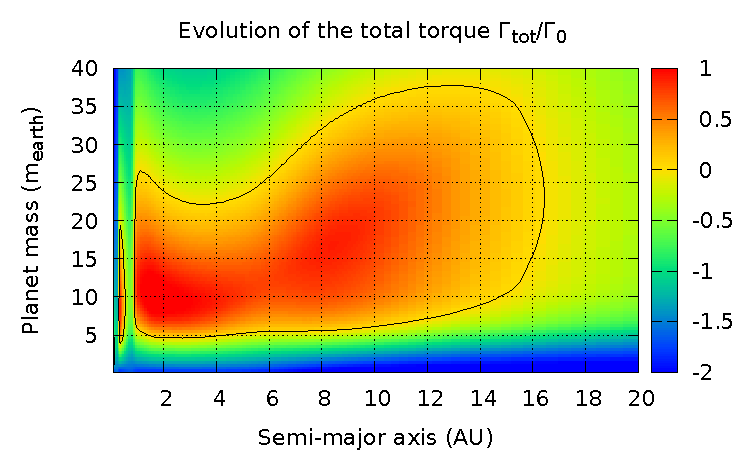
\includegraphics[width=0.49\textwidth]{figure/migration_map/TTauri/R_40_T_2850.pdf}}
\caption[Influence du rayon stellaire sur la carte de migration à flux stellaire constant.]{Influence du rayon $R_\star$ de
l'étoile centrale sur la carte de migration tandis que la luminosité de l'étoile est
conservée en variant la température. \refdisk}\label{fig:map_TTauri_radius}
\end{figure}

Le rayon plus grand $R\sim 2.5R_\odot$ des TTauri par rapport à des étoiles plus âgées \reffig{fig:TTauri_sample} tend à atténuer les régions ombrées (\og self-shadowing\fg) du disque. Au cours de son évolution, une étoile TTauri se contracte. À mesure que son rayon diminue, des ombres pourraient donc apparaître dans le disque, modifiant brutalement la carte de migration qui évoluait via la dissipation du disque.

\section{Influence de la viscosité du disque}
\subsection{Viscosité constante}\label{sec:nu_constant}

\begin{figure}[htbp]
\centering
\subfloat[$\nu=10^{14}\unit{cm^2/s}$]{\label{fig:nu_1e14}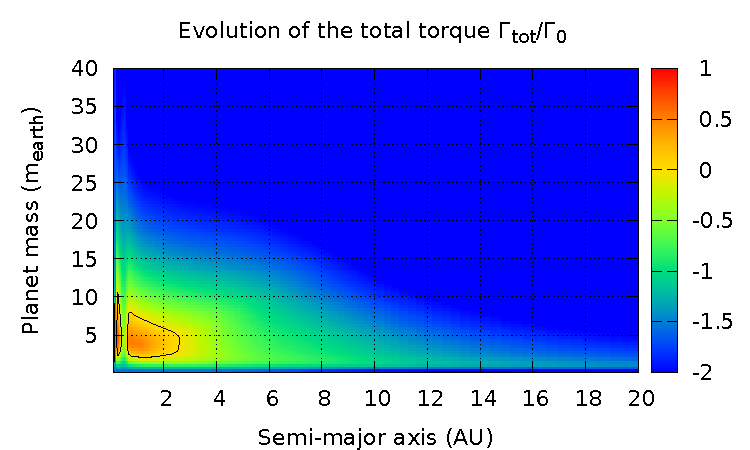
\includegraphics[width=0.49\textwidth]{figure/migration_map/viscosity/constant_1e14.pdf}}
\hfill
\subfloat[$\nu=5\cdot 10^{14}\unit{cm^2/s}$]{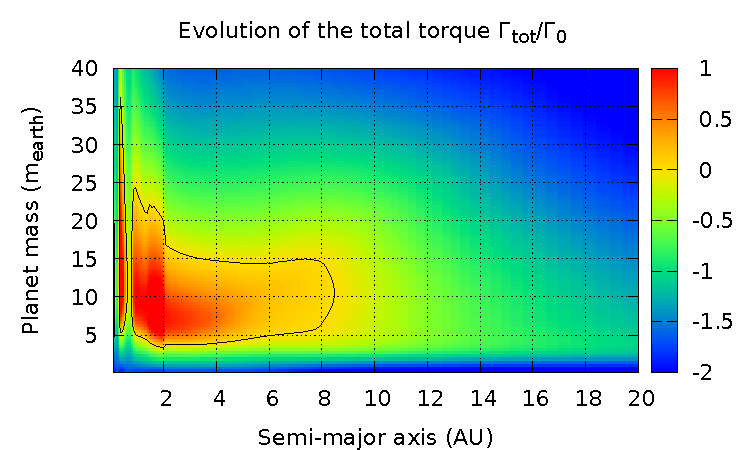
\includegraphics[width=0.49\textwidth]{figure/migration_map/viscosity/constant_5e14.pdf}}


\subfloat[$\nu=10^{15}\unit{cm^2/s}$]{\label{fig:nu_1e15}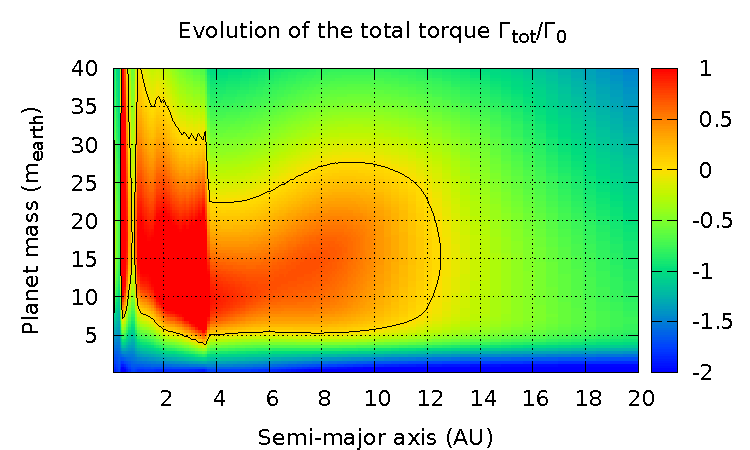
\includegraphics[width=0.49\textwidth]{%
figure/migration_map/viscosity/constant_1e15.pdf}}\hfill
\subfloat[$\nu=5\cdot 10^{15}\unit{cm^2/s}$]{\label{fig:nu_5e15}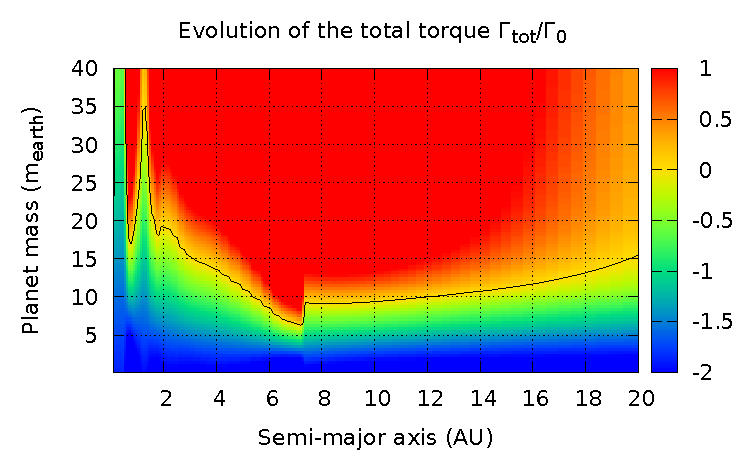
\includegraphics[width=0.49\textwidth]{figure/migration_map/viscosity/constant_5e15.pdf}}
\caption[Influence de la viscosité sur la carte de migration.]{Influence de la viscosité sur la carte de migration.
\refdisk}\label{fig:constant_viscosity}
\end{figure}

Le couple de migration est sensible à la valeur de la viscosité $\nu$ \reffig{fig:constant_viscosity}. À mesure que la
viscosité augmente, le chauffage visqueux en fait autant. La température augmente de manière générale dans le disque. Les
zones de migration vers l'extérieur se dilatent en même temps qu'elle se déplacent dans les parties externes du disque. Les
transitions d'opacité se déplacent également vers l'extérieur. 

De plus la viscosité agit sur la saturation du couple de corotation.
Quand la viscosité augmente, le temps de diffusion visqueux $t_\text{visc}$ diminue. Le couple de corotation ne sature pas tant
que $(t_\text{visc} < t_\text{lib}/2)$. Si on augmente la viscosité $\nu$, le couple de corotation sature moins facilement à
mesure que la masse de la planète augmente. La partie supérieure de la carte de migration se décale vers le haut quand la
viscosité augmente. 

Mais l'augmentation de la viscosité a un effet indirect sur le temps de diffusion radiatif $t_\text{rad}$. Si la viscosité augmente, le chauffage visqueux augmente. La température augmente, et la diffusivité thermique $\chi$ avec. Ainsi, quand la viscosité augmente, le temps de diffusion radiatif $t_\text{rad}$ diminue. Le couple de corotation est linéaire quand $t_\text{rad} < t_\text{U-turn}$. Quand la viscosité $\nu$ augmente, le couple de corotation se linéarise plus rapidement à mesure que la masse de la planète diminue. La partie inférieure de la carte de migration se décale elle aussi vers le haut. Des planètes de faible masse qui migraient vers l'extérieur ne peuvent plus migrer que vers l'intérieur à mesure que la viscosité augmente. 

\subsection{Viscosité alpha}\index{prescription alpha}
La prescription alpha \citep{shakura1973black} est une autre manière de définir la viscosité, à partir d'un paramètre adimensionné $\alpha$ \refsec{sec:viscosite-alpha}.

\begin{figure}[htbp]
\centering
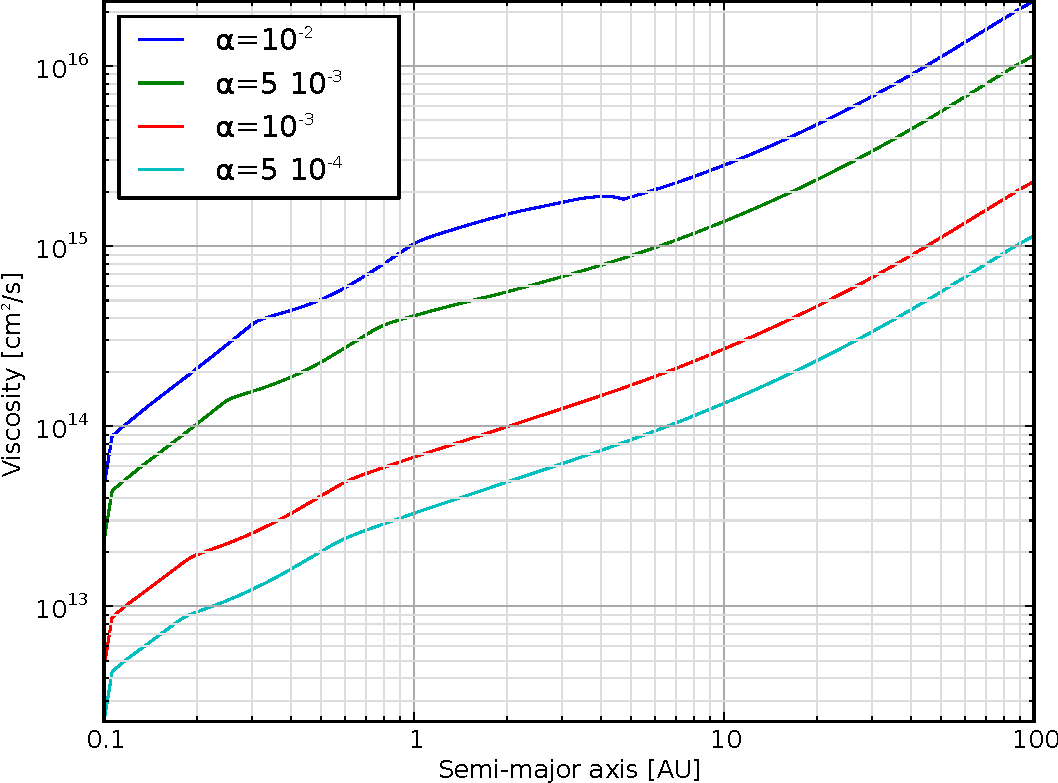
\includegraphics[width=0.6\linewidth]{figure/migration_map/viscosity/alpha_profiles.pdf}
\caption[Profils de viscosité dans le disque pour différentes valeurs de alpha.]{Profils de viscosité du disque en fonction de
la valeur de alpha. Ces profils correspondent à chacune des quatre cartes de migration
présentées \protect\reffig{fig:alpha_viscosity}. \refdisk}\label{fig:alpha_profiles}
\end{figure}

Par rapport à un modèle où la viscosité est constante, la prescription alpha entraine une augmentation continue de la viscosité en fonction de la distance \reffig{fig:alpha_profiles}. Pourtant ce n'est pas un simple facteur multiplicateur de la viscosité en raison du fait qu'il y a maintenant une dépendance en température au travers de l'échelle de hauteur et la vitesse du son. Les variations de $\alpha$ peuvent ainsi faire apparaître des transitions d'opacités au sein même du profil de viscosité. 

\begin{figure}[htbp]
\centering
\subfloat[$\alpha=10^{-2}$]{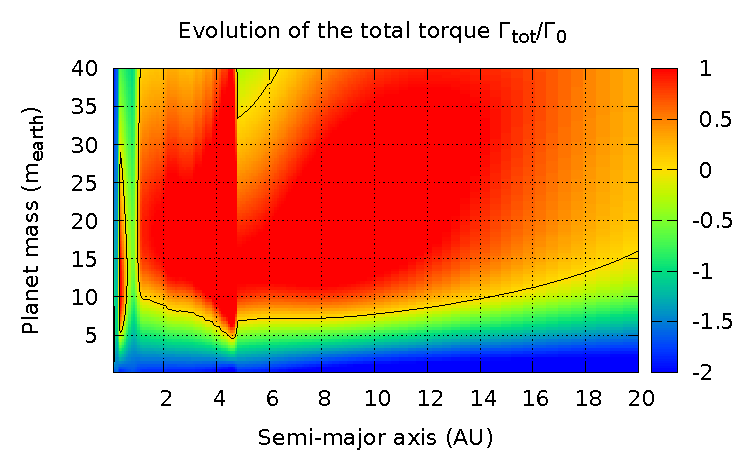
\includegraphics[width=0.49\textwidth]{figure/migration_map/viscosity/alpha_1e-2.pdf}}
\hfill
\subfloat[$\alpha=5\cdot 10^{-3}$]{\label{fig:alpha_5e-3}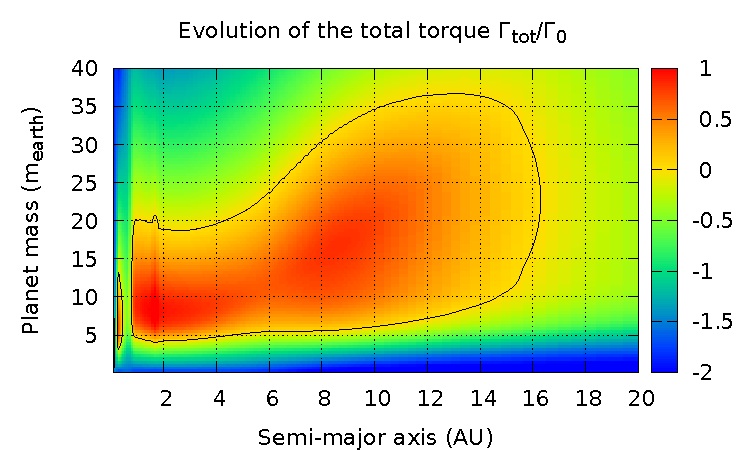
\includegraphics[width=0.49\textwidth]{figure/migration_map/viscosity/alpha_5e-3.pdf}}

\subfloat[$\alpha=10^{-3}$]{\label{fig:alpha_1e-3}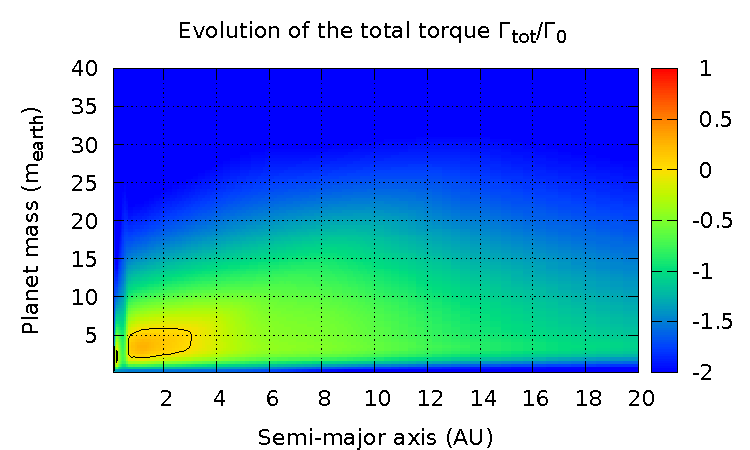
\includegraphics[width=0.49\textwidth]{%
figure/migration_map/viscosity/alpha_1e-3.pdf}}\hfill
\subfloat[$\alpha=5\cdot
10^{-4}$]{\label{fig:alpha_5e-4}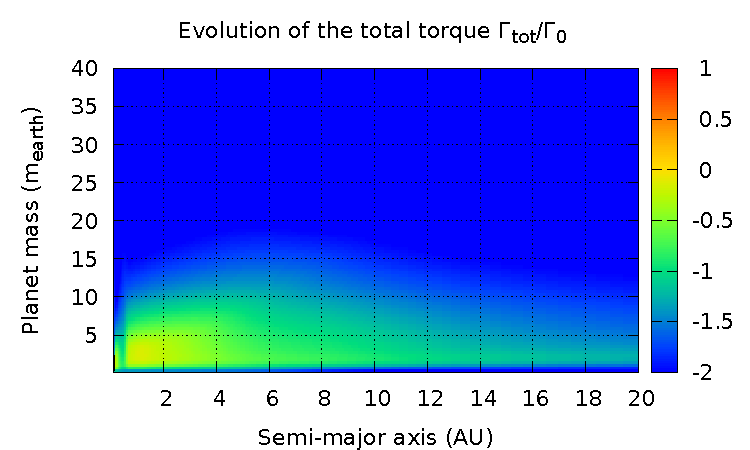
\includegraphics[width=0.49\textwidth]{figure/migration_map/viscosity/alpha_5e-4.pdf}}
\caption[Influence de alpha sur la carte de migration.]{Influence de la valeur de $\alpha$ dans le cadre d'une prescription
alpha pour la viscosité. \refdisk}\label{fig:alpha_viscosity}
\end{figure}

On fait varier la valeur de $\alpha$ dans une plage de valeurs tirée des observations \citep{guilloteau2011dual}. Dans les
disques jeunes, $\alpha$ peut atteindre $10^{-2}$, tandis que les disques un peu plus âgés \cite[fig.
16]{guilloteau2011dual} montrent des valeurs plus basses. Nous prenons comme plage de valeurs à étudier $\alpha\in[5\cdot
10^{-4} ; 10^{-2}]$. 

Pour une valeur de alpha donnée, la viscosité varie à travers le disque. Si on prend l'exemple de $\nu=10^{14}\unit{cm^2/s}$ \reffig{fig:nu_1e14}, cette viscosité est atteinte à $0.2\unit{UA}$ pour notre disque de référence avec $\alpha=5\cdot 10^{-3}$. La carte de migration dans cette région, autour de $0.2\unit{UA}$ est similaire dans le cas de la viscosité constante ou du modèle alpha. On remarque la même chose si on s'intéresse maintenant à $\nu=10^{15}\unit{cm^2/s}$ \reffig{fig:nu_1e15}, ce qui correspond à la zone autour de $6\unit{UA}$ pour notre disque de référence \reffig{fig:alpha_5e-3}.

Par contre, si nous cherchons à comparer $\nu=5\cdot 10^{15}\unit{cm^2/s}$ \reffig{fig:nu_5e15} avec le modèle $\alpha=5\cdot 10^{-3}$ \reffig{fig:alpha_5e-3} nous ne constatons aucune zone où la carte de migration est similaire. Le fait est que cela correspond à la zone autour de $45\unit{UA}$, région dans laquelle l'irradiation domine. Nous voyons donc qu'à viscosité équivalente, nous ne pouvons comparer un modèle alpha avec un modèle à viscosité constante uniquement dans les régions actives du disque, là où le chauffage visqueux domine. En effet, dans ces régions là, la viscosité étant l'origine principale de la température, c'est elle qui gouverne la carte de migration. 

Enfin, les cartes où $\alpha$ est très faible \reffig{fig:alpha_1e-3} et \reffig{fig:alpha_5e-4} montrent qu'à mesure que alpha
diminue, la viscosité fait de même de manière globale dans le disque. Dans ces disques là, on constate la disparition
progressive de la totalité des zones de convergences. Ainsi, dans le disque où alpha est le plus faible ($\alpha=5 10^{-4}$),
toutes les planètes migrent vers l'intérieur \reffig{fig:alpha_5e-4}, quelle que soit leur masse ou leur position dans le
disque.

\subsection{Dead zone}\index{zone morte}
\begin{figure}[htbp]
\centering
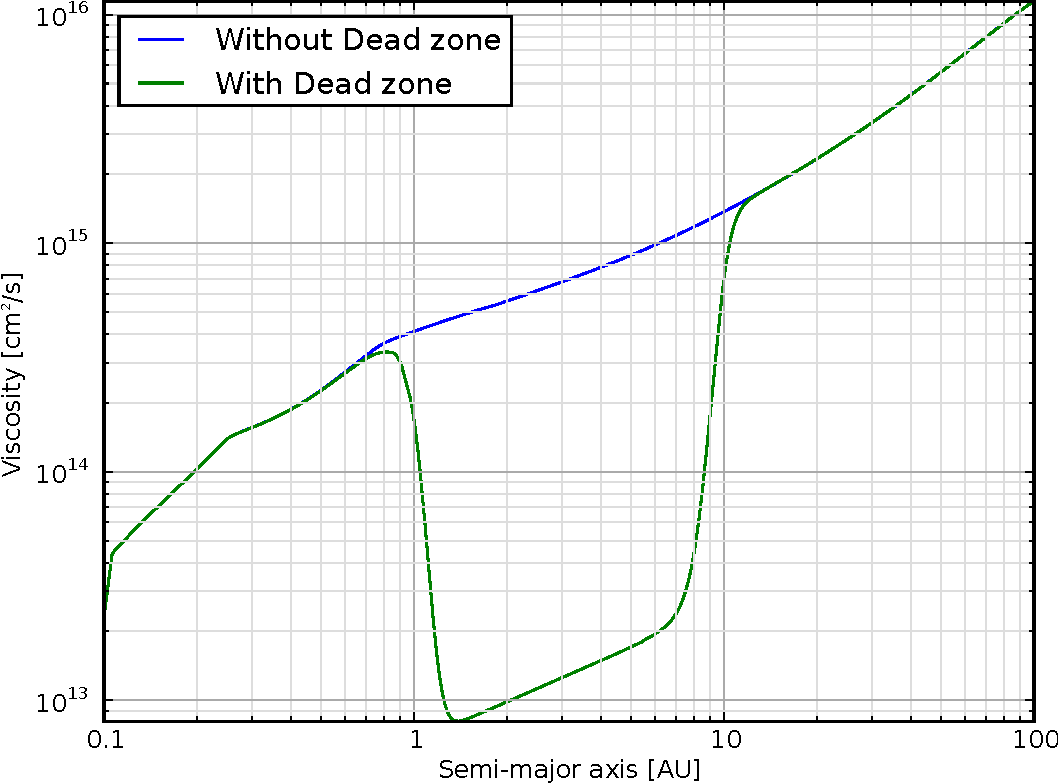
\includegraphics[width=0.6\linewidth]{figure/migration_map/viscosity/dead_zone_profile.pdf}
\caption[Effet d'une zone morte sur la viscosité.]{Profils de viscosité du disque selon qu'une zone morte est modélisée ou pas.
En dehors de la zone morte $\alpha=5\cdot 10^{-3}$. Dans la zone morte, $\alpha=10^{-4}$. Ces profils correspondent à chacune
des deux cartes de migration
présentées \protect\reffig{fig:viscosity_DZ}. \refdisk}\label{fig:dead_zone_profile}
\end{figure}

Une zone morte, ou \og dead zone\fg est une région d'un disque protoplanétaire où la turbulence est faible en raison d'un taux
d'ionisation extrêmement bas empêchant tout couplage du gaz du disque avec le champ magnétique de l'étoile
\refsec{sec:ionisation_DZ}.

Dans la zone morte, la viscosité chute rapidement, et augmente en fonction de la distance dans un régime différent que dans le reste du disque \reffig{fig:dead_zone_profile}. 

\begin{figure}[htbp]
\centering
\subfloat[Sans dead zone]{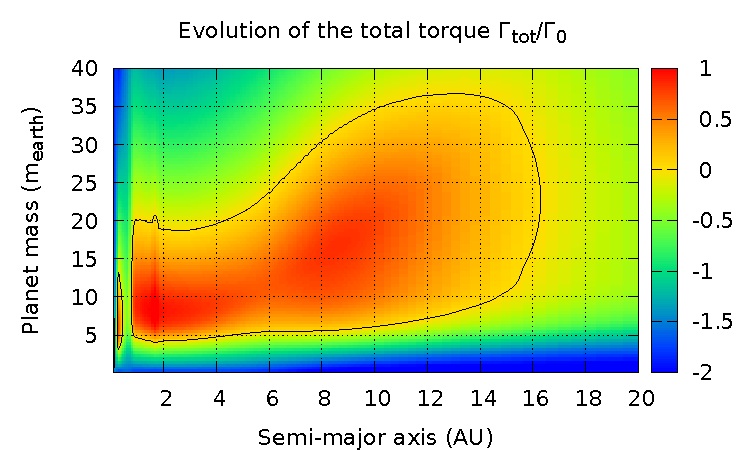
\includegraphics[width=0.49\textwidth]{figure/migration_map/viscosity/alpha_5e-3.pdf}}\hfill
\subfloat[Avec dead zone]{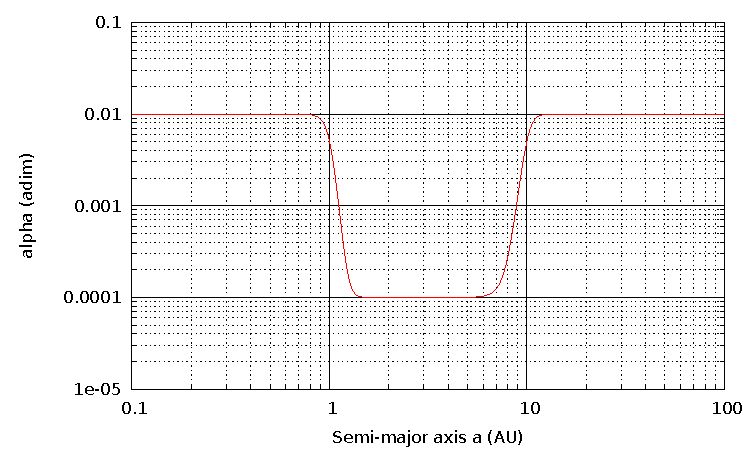
\includegraphics[width=0.49\textwidth]{%
figure/migration_map/viscosity/alpha_dz.pdf}}

\caption[Effet d'une zone morte sur la carte de migration.]{Effet d'une zone morte sur la carte de migration. Au cœur de la dead
zone, $\alpha=10^{-4}$. En dehors, $\alpha=5\cdot 10^{-3}$. Dans les zones de transitions, la valeur de $\alpha$ est lissée. La
zone morte s'étend de $1$ à $10\unit{UA}$. Plus de détails sur la modélisation de la zone morte \protect\refsec{sec:dead_zone}.
\refdisk}\label{fig:viscosity_DZ}
\end{figure}

Sur les cartes de migration \reffig{fig:viscosity_DZ}, l'entrée dans la dead zone modifie en profondeur la carte de migration en creusant une zone de migration vers l'intérieur en raison de la viscosité très faible. Le temps de diffusion visqueux $t_\text{visc}$ augmente alors brusquement, engendrant la saturation rapide du couple de corotation quelle que soit la masse de la planète. Ainsi, dans la zone morte, la possibilité de migration vers l'extérieur est fortement réduite. En dehors de la zone morte, la carte de migration est quasi inchangée.

\bigskip

Maintenant, on cherche à voir l'effet conjoint d'une zone morte et de l'ombre du disque modélisée de manière complexe (\textbf{modèle étendu}) dans \refsec{sec:shadow}.

Au bord interne de la zone morte, où le chauffage visqueux domine, la brusque diminution de la viscosité entraine une diminution de la température, l'irradiation de l'étoile devient temporairement dominante par rapport au chauffage visqueux. Comme nous l'avions vu en fin de \refsec{sec:shadow} l'effet de l'ombre ne devient important que dans les parties passives du disque, ce qu'est le bord interne de la zone morte à cause de la brusque diminution de la viscosité. Ainsi, au bord interne de la zone morte, l'ombre du disque joue un rôle important \reffig{fig:dz_shadow_temp}. Elle fait apparaître une zone de convergence pour les planètes de faibles masses qui autrement migrent vers l'intérieur \reffig{fig:dz_shadow_map}.

\begin{figure}[htbp]
\centering
\subfloat[Carte de migration]{\label{fig:dz_shadow_map}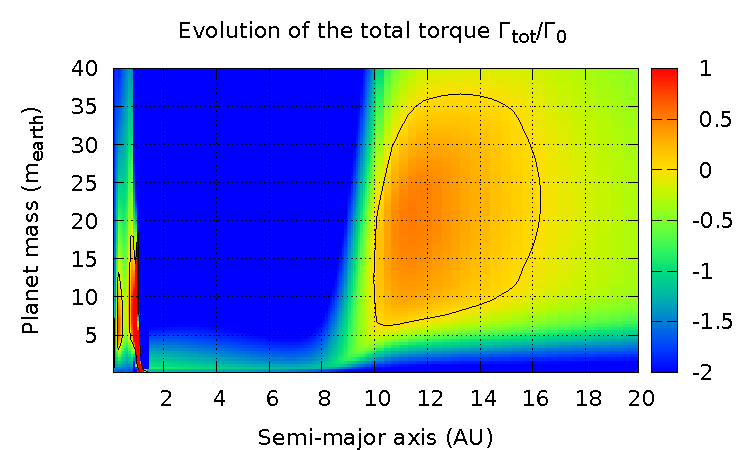
\includegraphics[width=0.49\textwidth]{figure/migration_map/viscosity/dz_shadow.pdf}}\hfill
\subfloat[Profil de température]{\label{fig:dz_shadow_temp}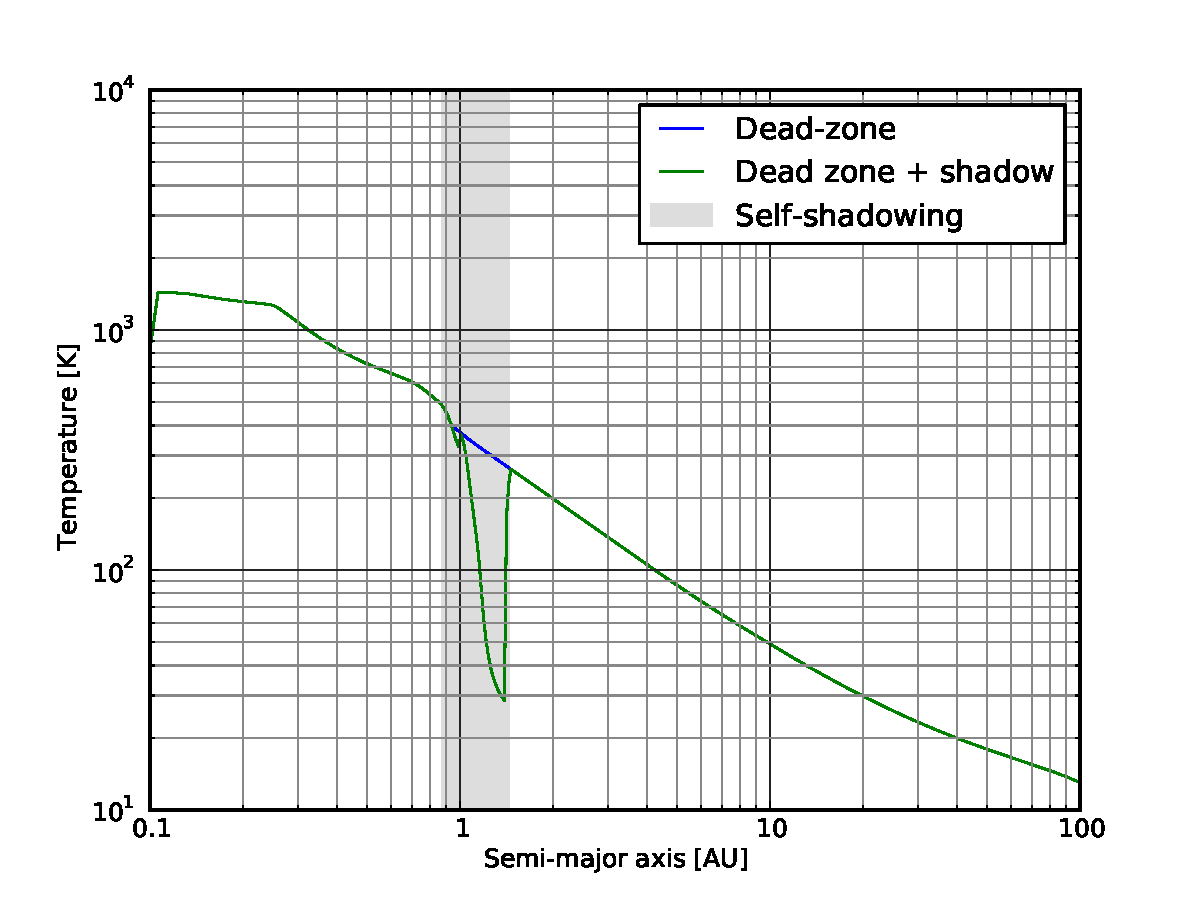
\includegraphics[width=0.49\textwidth]{%
figure/migration_map/viscosity/dz_shadow_temp_profile.pdf}}

\caption[Effets conjoint d'une zone morte et du self-shadowing sur la carte de migration.]{Effet conjoint d'une zone morte et du
\og self-shadowing\fg. La zone morte s'étend de $1$ à $10\unit{UA}$. Plus de détails sur la modélisation de la zone morte
\protect\refsec{sec:dead_zone}. \refdisk}\label{fig:dz_shadow}
\end{figure}

Cette soudaine chute de la température entraine une augmentation du temps de diffusion radiatif $t_\text{rad}$. Cette augmentation du temps de diffusion rend beaucoup plus difficile pour le couple de corotation de tendre vers sa valeur linéaire. Même pour des masse de planète faibles, le couple de corotation est non-linéaire et fait apparaître une zone de migration vers l'extérieur au début de la zone morte, peu après $1\unit{UA}$. 

Cette zone de convergence sera sans doute très intéressante au niveau de l'accrétion de masse et de la formation des
planètes car peu étendue, mais elle pourrait malgré tout jouer un rôle majeur en maintenant des planètes telluriques de faibles
masses (de l'ordre de $1\mearth$) dans le disque, sans besoin d'aucun compagnon massif en résonance pour la maintenir.

La modélisation poussée de l'ombre du disque et son effet sur l'irradiation pourrait donc jouer un rôle majeur au niveau des
zones mortes où une zone locale où l'irradiation domine apparaît dû à la décroissance soudaine de la viscosité et du chauffage
qui en découle \citep{matsumura2003origin}.

\section{Profil de densité de surface}
Dans notre modèle, le profil de la densité de surface est notre plus grande incertitude. Les contraintes observationnelles ne
restreignent pas suffisamment le profil de densité \citep[Fig. 12]{mundy2000structure, andrews2007high, williams2011protoplanetary,
guilloteau2011dual}. C'est à partir de ce profil de densité de surface que nous calculons toutes les propriétés du disque, en
particulier la température et l'échelle de hauteur, puis la migration des planètes. 

On définit la loi de puissance pour la densité de surface de la façon suivante : 
\begin{align}
\Sigma(R) &= \Sigma_0 * \left(\frac{R}{R_0}\right)^{-d}
\end{align}
où $\Sigma_0$ est la densité de surface à $R_0=1\unit{UA}$.

À l'instar de
la viscosité $\nu$, le profil de densité de surface $\Sigma$ influence directement le chauffage visqueux. Cependant, changer la
densité de surface permet de modifier le chauffage visqueux sans modifier le temps de diffusion visqueux $t_\nu$. Je cherche à
étudier l'influence de l'indice $d$ de la loi de puissance sur la carte de migration, soit en le faisant varier
individuellement, soit en regardant, à masse du disque constante, ce que le profil de densité change. 

\subsection{Variation de l'indice d}\label{sec:sigma_index}
\begin{figure}[htbp]
\centering
\subfloat[$d=0.6$]{\label{fig:d06}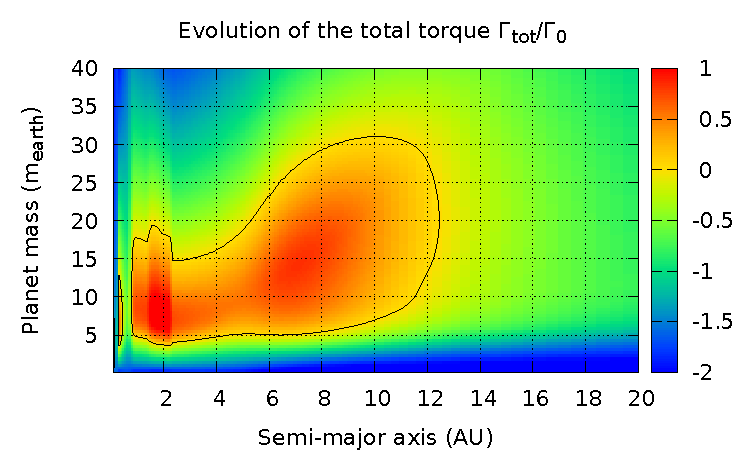
\includegraphics[width=0.49\textwidth]{%
figure/migration_map/index/sigma/300_06.pdf}}\hfill
\subfloat[$d=0.7$]{\label{fig:d07}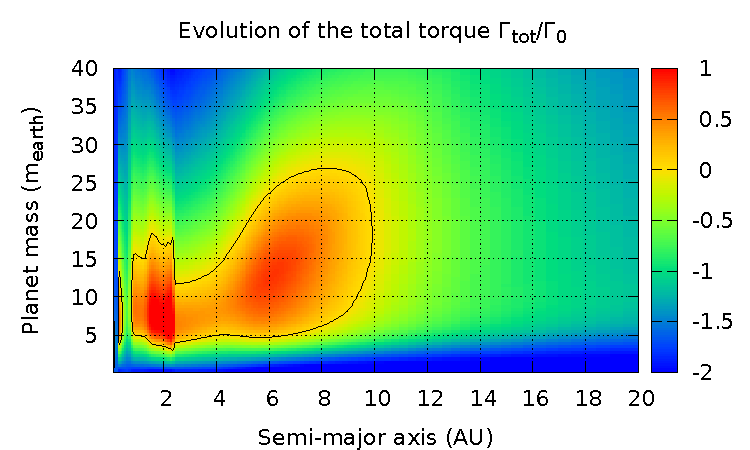
\includegraphics[width=0.49\textwidth]{figure/migration_map/index/sigma/300_07.pdf}}

\subfloat[$d=1$]{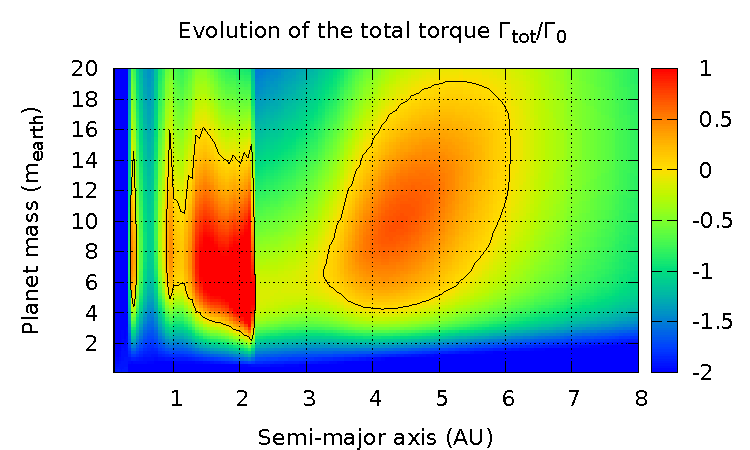
\includegraphics[width=0.49\textwidth]{%
figure/migration_map/index/sigma/300_10.pdf}}\hfill
\subfloat[$d=1.5$]{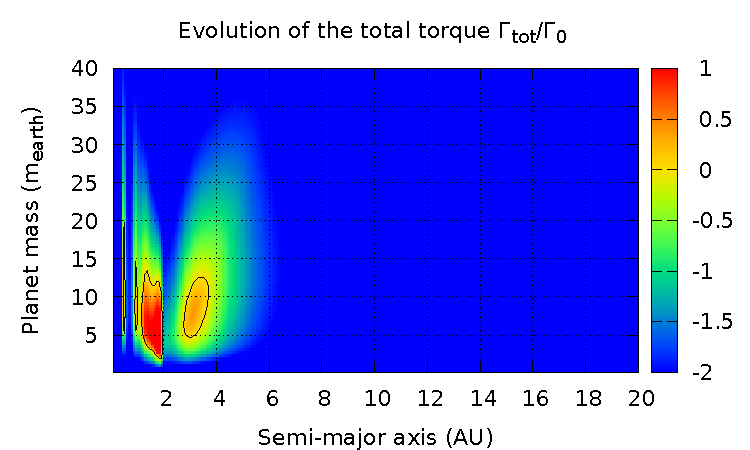
\includegraphics[width=0.49\textwidth]{figure/migration_map/index/sigma/300_15.pdf}}

\caption[Influence du profil de densité sur la carte de migration.]{Influence de l'indice $d$ de la loi de puissance définissant
la densité de surface du disque sur la carte de migration.
Ici, $\Sigma_0=\cte=300\unit{g/cm^2}$, seul l'indice $d$ du profil de densité de surface varie. \refdisk}\label{fig:map_index}
\end{figure}

Si l'indice $d$ du profil de densité de surface augmente, la forme de la carte de migration aura tendance à se compresser autour
du rayon $R_0=1\unit{UA}$ où est défini la densité $\Sigma_0$ \reffig{fig:map_index}. En effet, pour $\Sigma_0$ fixé, si on
augmente $d$, alors on augmente la masse du disque en dessous de $R_0$ tandis qu'on diminue sa masse au delà de $\Sigma_0$
\reffig{fig:index_density}. Cette modification de la masse joue sur le chauffage visqueux et donc sur le profil de température
qui décroit plus rapidement en fonction du rayon \reffig{fig:index_temp}. En dessous de $R_0$, la température est plus
importante à mesure que $d$ augmente. Au delà de $R_0$ c'est l'inverse. Dans les parties externes où le chauffage visqueux ne
joue aucun rôle, c'est l'irradiation qui détermine la température. La densité joue encore un rôle au travers de l'opacité dans
la partie passive du disque, jusqu'à ce que l'opacité ne dépende quasiment plus de la densité (à température faible
$T<100\unit{K}$).

\begin{figure}[htbp]
\centering
\subfloat[Profils de densité]{\label{fig:index_density}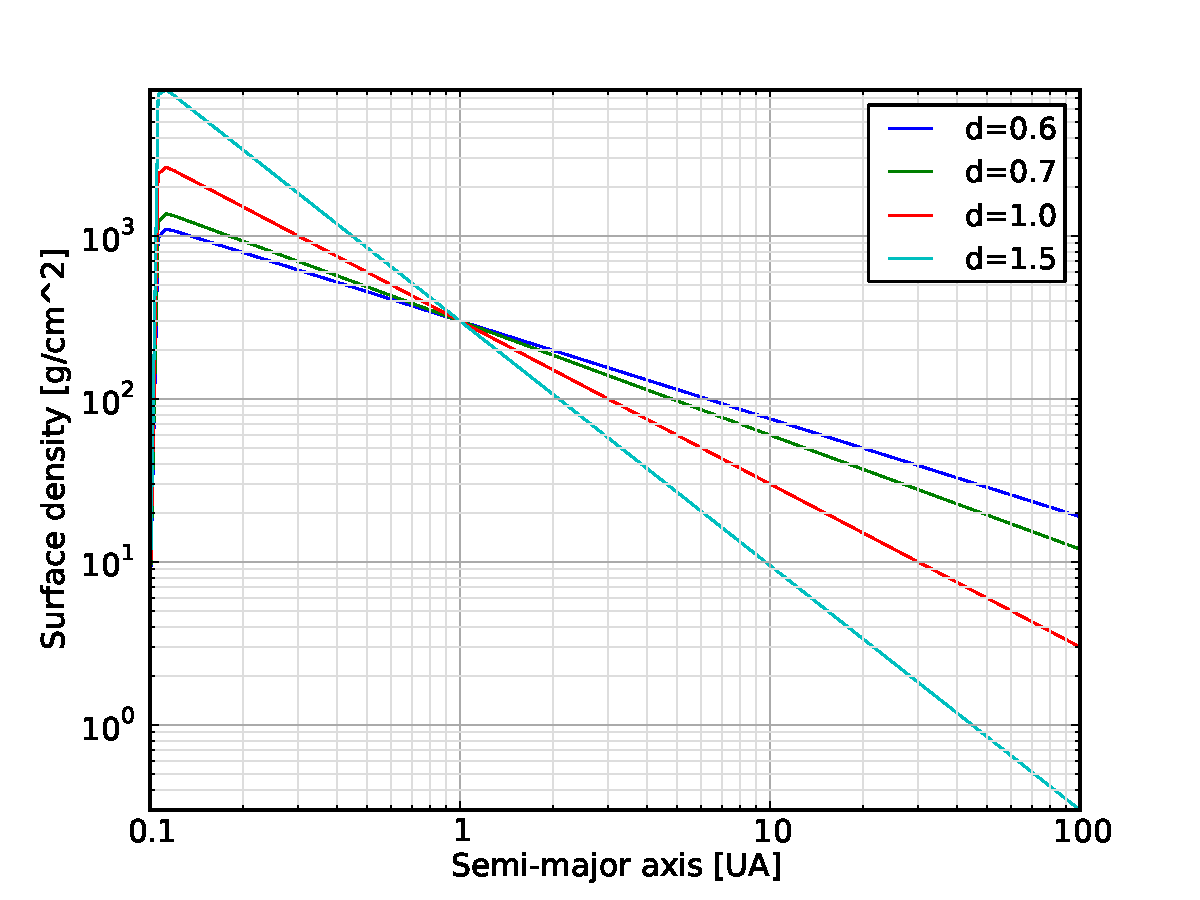
\includegraphics[width=0.49\textwidth]{%
figure/migration_map/index/sigma/density_profile.pdf}}\hfill
\subfloat[Profils de
température]{\label{fig:index_temp}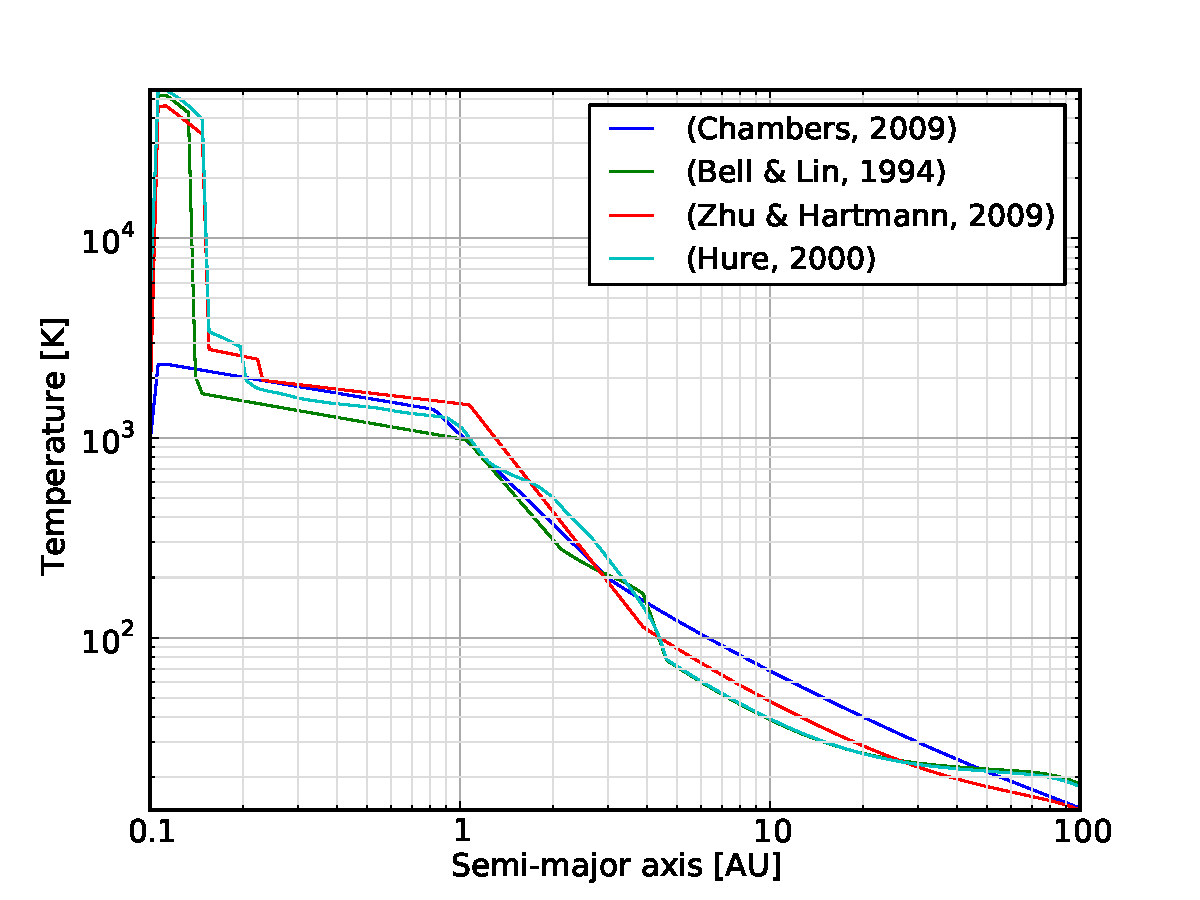
\includegraphics[width=0.49\textwidth]{%
figure/migration_map/index/sigma/temperature_profile.pdf}}

\caption{Profils de densité et température pour les 4 cartes de migration présentées
\protect\reffig{fig:map_index}.}\label{fig:index_profiles}
\end{figure}

\subsection{Dissipation du disque}\label{sec:sigma_0}\index{dissipation du disque}

\begin{figure}[htbp]
\centering
\subfloat[$\Sigma_0=1200\unit{g/cm^2}$]{\label{fig:1200_map}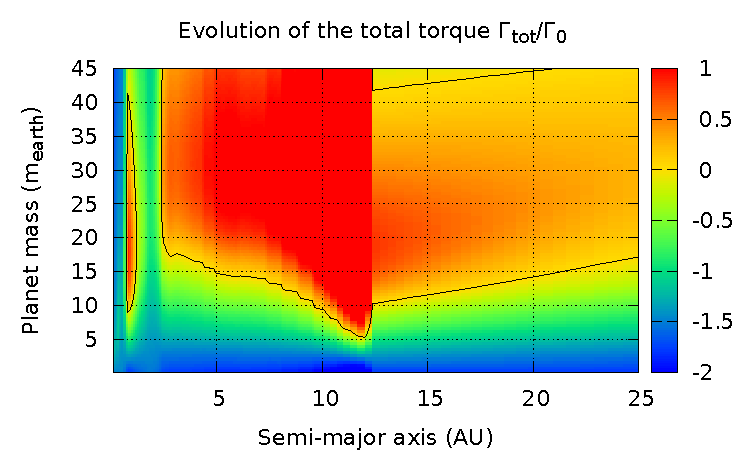
\includegraphics[width=0.49\textwidth]{%
figure/migration_map/total_mass/1200_05.pdf}}\hfill
\subfloat[$\Sigma_0=600\unit{g/cm^2}$]{\label{fig:600_map}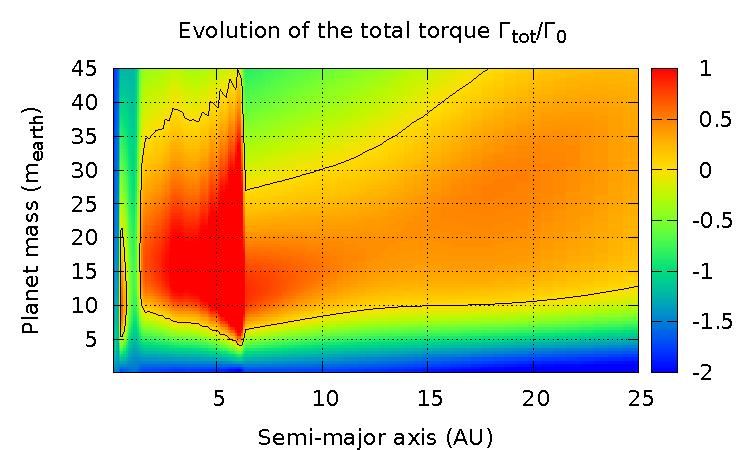
\includegraphics[width=0.49\textwidth]{%
figure/migration_map/total_mass/600_05.pdf}}

\subfloat[$\Sigma_0=300\unit{g/cm^2}$]{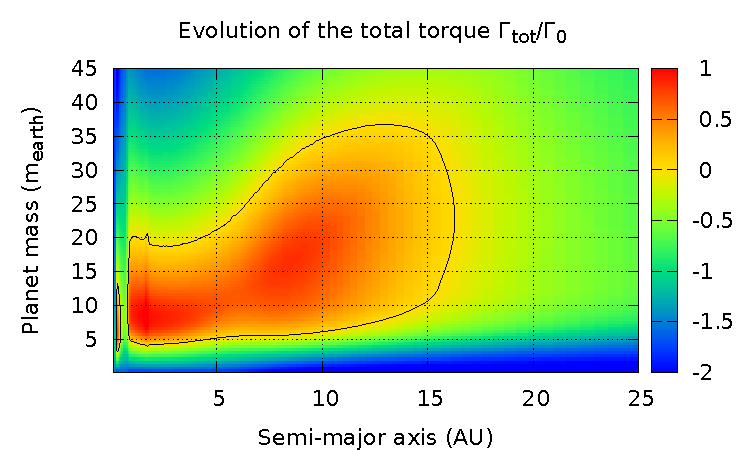
\includegraphics[width=0.49\textwidth]{%
figure/migration_map/total_mass/300_05.pdf}}\hfill
\subfloat[$\Sigma_0=150\unit{g/cm^2}$]{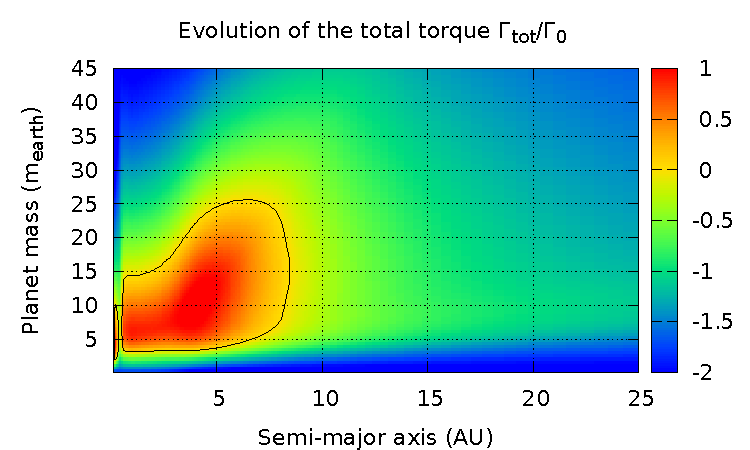
\includegraphics[width=0.49\textwidth]{%
figure/migration_map/total_mass/150_05.pdf}}

\caption[Effet de la dissipation sur la carte de migration.]{Par rapport au disque de référence, possédant un profil de densité
de surface $\Sigma(R) = 300 \cdot
R^{-\sfrac{1}{2}}\unit{g/cm^2}$ nous représentons les cartes de migration pour des disques où nous avons changé la masse. D'en haut à gauche vers en bas à droite, ces cartes représentent les premiers stades de la dissipation du disque. \refdisk}\label{fig:map_total_mass}
\end{figure}

Étudier l'influence de la masse du disque nous permet de remonter à l'effet de la dissipation du disque. En particulier dans la
première phase de la dissipation, quand le profil de densité de surface n'évolue pas beaucoup. Dans la seconde partie gouvernée
par la photo-évaporation, la dissipation ne conserve pas le profil en loi de puissance de la densité de surface (en faisant
l'approximation que ce dernier en est un initialement) \reffig{fig:disk_dispersion}. Au lieu de ça, le
disque va se creuser à partir d'un certain rayon, optimal vis à vis de la photo-évaporation. Le disque va alors se scinder en
deux, la partie interne va rapidement tomber sur l'étoile centrale et dans un dernier stade les parties externes vont aussi se
dissiper. Si les détails de la dissipation ne sont pas connus, il apparait malgré tout qu'une unique décroissance exponentielle
du disque tout au long de sa vie ne représente pas fidèlement l'évolution du disque \citep{alexander2006photoevaporation}. Dans
le cadre de la migration planétaire où les profils de densité et de températures jouent un rôle fondamental, nous nous limitons
donc à l'étude des premiers millions d'années d'évolution du disque. 

À l'instar de la viscosité, la densité de surface $\Sigma_0$ agit sur le chauffage visqueux et donc indirectement sur le temps de diffusion radiatif $t_\text{rad}$. Par contre, quand on augmente la densité, on ne modifie pas le temps de diffusion visqueuse qui influe sur la saturation. 

Ainsi, à partir du profil de référence avec $\Sigma(R) = 300 \cdot
R^{-\sfrac{1}{2}}\unit{g/cm^2}$ et $\alpha=5\cdot 10^{-3}$. Si on multiplie la densité par deux $\Sigma_0=600\unit{g/cm^2}$ ou qu'on double la valeur d'alpha $\alpha=10^{-2}$, le chauffage visqueux est le double de celui dans le disque de référence au premier ordre. Dans le cas où on a modifié la viscosité, la saturation du couple de corotation intervient à des masses de planètes plus importantes que dans le cas où la viscosité est resté la même ($\nu$ augmente, donc $t_\nu$ diminue).  

Une variation équivalente du chauffage visqueux entraine un disque globalement plus froid quand cette variation provient de la viscosité, contrairement à une variation de densité car cette dernière agit aussi indirectement sur l'opacité. 
Si on augmente la température, la diffusivité thermique est plus grande, le temps de diffusion radiatif $t_\text{rad}$ diminue. Le couple de corotation devient linéaire pour des masses plus grandes. 

Quand la densité diminue, on observe les mêmes effets qu'avec la diminution de la viscosité \reffig{fig:map_total_mass}, mais ces effets sont amplifiés car la densité influe sur l'opacité du disque. Le profil de température diminue plus rapidement. La carte de migration se compresse plus rapidement vers l'intérieur du disque en variant la densité (par opposition à une variation de viscosité). Par contre, la viscosité n'évoluant pas, la partie supérieure de la carte de migration se compresse moins rapidement vers le bas. Des planètes massives conserveront donc une zone de migration vers l'extérieur plus longtemps si on diminue la densité au lieu de diminuer la viscosité. On remarque que les deux disques les plus massifs présentent une transition d'opacité très marquée respectivement à $6$ \reffig{fig:600_map} et $12\unit{UA}$ \reffig{fig:1200_map}. 

\bigskip

On note enfin que lors de la dissipation du disque, les observations semblent montrer que la viscosité diminue \citep[fig. 16]{guilloteau2011dual}. La densité et la viscosité ayant le même genre d'effet sur la carte de migration, on s'attend à une compression rapide de la carte de migration. Les parties externes vont se rapprocher de l'étoile, c'est à dire que les planètes, quelles que soient leur masse vont avoir tendance à migrer moins loin dans le disque. Les planètes les plus massives qui pouvaient auparavant migrer vers l'extérieur ne pourront plus le faire à mesure que le disque se dissipe. 

À mesure que le disque se dissipe, la masse critique minimale pour qu'une planète puisse migrer vers l'extérieur diminue. Des planètes de faibles masses qui auparavant migraient inexorablement vers l'intérieur peuvent donc migrer vers l'extérieur. 

Une manière de résumer l'effet de la dissipation du disque sur la carte de migration, c'est de dire que la carte de migration
est compressée vers le coin en bas à gauche de la carte de migration, le point (0;0) dans le système de coordonnées (distance ;
masse).

\subsection{Variation du profil à masse totale constante}
On remarque que l'augmentation de l'indice $d$ du profil de densité de surface va avoir un impact sur la masse totale du
disque. Si on augmente $d$, la masse du disque diminue. On a vu précédemment que la masse du disque avait un effet inverse par rapport à l'indice $d$. Si on augmente
l'indice $d$, on compresse la zone de migration externe vers l'étoile centrale. Au contraire, si on augmente la masse totale, on
dilate cette zone radialement. 

\begin{table}[htbp]
\centering
\begin{tabular}{|c|c|c|c|}
\hline 
 & $d=0.5$ & $d=1.0$ & $d=1.5$ \\\hline 
$R\in[100 ; 1000]\unit{UA}$ & $300$ & $6805$ & $1.416\cdot 10^5$ \\ \hline 
$R\in[0.1 ; 100]\unit{UA}$ & $300$ & $2002$ & $10330$ \\ \hline 
$R\in[1 ; 20]\unit{UA}$ & $300$ & $931$ & $2547$ \\ \hline 
$R\in[2 ; 4]\unit{UA}$ & $300$ & $517$ & $883$ \\ \hline 
\end{tabular} 
\caption[Différents profils de disque ayant la même masse totale.]{Valeur de la densité en \unit{g/cm^2} à $R_0=1\unit{UA}$
qu'il faut choisir en fonction de la valeur de $d$ pour avoir une masse de disque identique dans la gamme de distance orbitale
choisie.}\label{tab:profils_equivalents}
\end{table}

On cherche maintenant à étudier l'influence du profil de densité de surface quand on cherche à garder la masse du disque constante. La masse d'un anneau de matière de largeur $\dif R$ est donnée par : 
\begin{align}
\dif M(R) &= 2\pi \Sigma_0 R^{1-d} \dif R
\end{align}
où $d$ est l'opposé de l'indice de la loi de puissance pour la densité. 

Cela signifie qu'en fonction de l'indice $d$ du profil, la masse du disque sera uniformément répartie ($d=1$), concentrée au bord interne ($d>1$) ou concentrée au bord externe du disque ($d<1$). 

Dit autrement, cela signifie que les bornes que l'on choisi pour calculer la masse du disque ne sont pas neutres. En choisissant pour référence le profil : 
\begin{align}
\Sigma(R) &= \Sigma_0 \times R^{-0.5}
\end{align}
\reftab{tab:profils_equivalents} récapitule les différents profils que nous devrions choisir pour avoir la même masse, en fonction des bornes que l'on considère pour la normalisation de la masse. 

\begin{figure}[htbp]
\centering
\subfloat[$d=1$ ; $\Sigma_0=2000\unit{g/cm^2}$]{\includegraphics[width=0.49\textwidth]{%
figure/migration_map/index/mass/01_100/2000_10.pdf}}\hfill
\subfloat[$d=1.5$ ;
$\Sigma_0=10000\unit{g/cm^2}$]{\includegraphics[width=0.49\textwidth]{figure/migration_map/index/mass/01_100/10000_15.pdf}}

\caption[Cartes de migration pour différents profils de densité extrêmes, la masse du disque étant la même entre 0.1 et 100
UA.]{Cartes de migration pour différents profils pour lesquels la masse du disque est constante entre $R=0.1\unit{UA}$ et
$R=100\unit{UA}$. La densité locale est la même pour $R=27\unit{UA}$. \refdisk}\label{fig:map_mtot_01_100}
\end{figure}

Dans \reffig{fig:map_mtot_01_100}, la densité des deux profils est la même à $27\unit{UA}$. Nous remarquons que la carte de migration est décalée plus loin dans le disque. Ceci est dû au fait que nous sommes à l'intérieur du rayon $R=27\unit{UA}$ pour lequel les densités sont égales. En dessous de ce rayon, quand $d$ augmente, la densité augmente. Ainsi, le profil en $R^{-1.5}$ est beaucoup plus massif. La température est donc plus importante. À ce titre, notons tout de même que la température au bord interne est dans ce cas précis supérieure à \nombre{100000} K. Ces profils sont extrêmes et ne représentent pas des disques réalistes. C'est dû au fait que nous cherchons à conserver la masse dans une gamme de distance importante. Les profils concentrant la masse soit à l'intérieur soit à l'extérieur, les disparités entre les profils sont accentuées d'autant. 

\begin{figure}[htbp]
\centering
\subfloat[$d=1$ ; $\Sigma_0=517\unit{g/cm^2}$]{\includegraphics[width=0.49\textwidth]{%
figure/migration_map/index/mass/2_4/517_10.pdf}}\hfill
\subfloat[$d=1.5$ ;
$\Sigma_0=883\unit{g/cm^2}$]{\includegraphics[width=0.49\textwidth]{figure/migration_map/index/mass/2_4/883_15.pdf}}

\caption[Cartes de migration pour différents profils de densité, la masse du disque étant la même entre 2 et 4 UA.]{Cartes
de migration pour différents profils pour lesquels la masse du disque est constante entre $R=2\unit{UA}$ et $R=4\unit{UA}$. La
densité locale est environ la même autour de $R=3\unit{UA}$ par rapport au disque de référence. 
\refdisk}\label{fig:map_mtot_2_4}
\end{figure}

Si nous cherchons maintenant à conserver la masse non pas entre $0.1$ et $100\unit{UA}$ comme précédemment, mais entre $2$ et $4\unit{UA}$, nous obtenons les cartes de migrations \reffig{fig:map_mtot_2_4}. Ici, la distance de l'étoile où la masse locale du disque est la même quel que soit le profil est à $R=3\unit{UA}$. Ce rayon est alors la distance de référence autour de laquelle la carte de migration se comprime. En effet, quand $d=1.5$ la densité de surface varie beaucoup plus rapidement que dans le cas $d=1$, l'effet net est alors de conserver en première approximation la carte de migration, mais de la comprimer autour de la distance de référence, ici $R=3\unit{UA}$.

\begin{figure}[htbp]
\centering
\subfloat[$d=0.6$ ; $\Sigma_0=444\unit{g/cm^2}$]{\label{fig:d06iso}\includegraphics[width=0.49\textwidth]{%
figure/migration_map/index/mass/01_100/444_06.pdf}}\hfill
\subfloat[$d=0.7$ ;
$\Sigma_0=653\unit{g/cm^2}$]{\label{fig:d07iso}\includegraphics[width=0.49\textwidth]{figure/migration_map/index/mass/01_100/653_07.pdf}}

\caption[Influence de l'indice d pour la densité de surface (à masse constante) sur la carte de migration.]{Influence de
l'indice $d$ du profil de densité de surface tout en maintenant la masse totale du disque constante pour
$R\in[0.1;100]\unit{UA}$.
\refdisk}\label{fig:map_index_mtot}
\end{figure}

Enfin, \reffig{fig:map_index_mtot} montre deux cartes de migrations où la masse est conservée entre $0.1$ et $100\unit{UA}$ mais pour lesquelles l'indice $d$ a été très peu modifié. Dans ce cas là, la masse locale du disque est égale pour les deux profils à $R=48\unit{UA}$. 

\bigskip

En résumé, quand on change l'indice $d$ du profil de densité, il faut définir le rayon auquel les densités des deux profils sont égales pour interpréter la carte de migration. En dessous de cette distance, la masse locale du profil le plus abrupt sera la plus grande, et inversement dans les parties externes. Ainsi, on se ramène à l'interprétation en terme de masse locale que nous avions utilisée pour étudier la dissipation du disque. C'est l'effet le plus important que la densité de surface apporte, car elle influe directement sur le profil de température. Les variations du couple de migration induites directement par la valeur de $d$ restent en deçà des variations indirectes via la température. En effet la diffusivité thermique $\chi$ a une dépendance en $T^3$ (voir \refeq{eq:diffusivity}, $H^2\propto T$).

\section{Autres paramètres}
\subsection{Table d'opacité}\label{sec:influence_opacity_table}\index{opacité}
Nous l'avons vu dans les parties précédentes, le profil de température est crucial pour évaluer la migration dans le disque. La densité a notamment un effet indirect sur la température au travers de l'opacité. Nous allons maintenant montrer que le choix du modèle a une influence considérable sur la migration, le modèle choisi pour l'opacité étant une source importante d'incertitude.

Dans toute la suite, quand je parlerai de table d'opacité, je désigne le fait d'utiliser un tableau à deux dimensions,
proposant des valeurs de l'opacité pour différentes températures et densités. La table d'opacité est donc définie ici par
opposition à ce que j'appelle des lois d'opacité, modèles dans lesquels l'opacité est définie par des lois de puissance,
fonction de la température et de la densité, dans différents régimes de température et densité.

Ainsi une table d'opacité est simplement une tabulation de l'opacité, alors qu'une loi d'opacité correspond à un ajustement d'une table d'opacité par
une ou plusieurs lois de puissance. 

\bigskip

Généralement, c'est la loi d'opacité \cite{bell1994FU} qui est utilisée, aussi bien dans les simulations hydrodynamiques 2D et
3D que dans les simulations N-corps. 

Une autre loi d'opacité existante est \cite{zhu2009nonsteady}, loi quelque peu améliorée par rapport à \cite{bell1994FU},
l'augmentation des capacités des ordinateurs ayant permis de faire des calculs plus précis. 

De plus, nous utilisons aussi le modèle d'opacité très simple décrit par \cite{chambers2009analytic} dans lequel l'opacité est
constante et égale à $\kappa=3$ jusqu'à $1380\unit{K}$ où une transition s'opère vers une loi de puissance pour les hautes températures. Ce modèle nous
permet de voir l'effet d'un modèle par rapport à un cas où l'opacité est constante. En effet, dans le cas d'un disque
protoplanétaire, seules les régions les plus internes sont susceptibles d'atteindre des températures supérieures à
$1000\unit{K}$. 

Enfin, j'ai souhaité comparer ces deux lois d'opacité avec une table d'opacité, \cite{hure2000transition} \reffig{fig:hure_profile}. Cette table
d'opacité de Rosseland correspond à la composition suivante $X=0.70$, $Y=0.28$ et $Z=0.02$ et est basée sur
\cite{seaton1994opacities, alexander1994low, henning1996dust}.

\begin{figure}[htbp]
\centering
\includegraphics[width=0.65\linewidth]{figure/hure_opacity_table.pdf}
\caption[Représentation de la table d'opacité \cite{hure2000transition}.]{Représentation de la table d'opacité
\cite{hure2000transition} dans des coordonnées qui permettent d'obtenir une bonne précision lors de l'interpolation. Ici,
$\log(R)=\log(\rho) + 18 -3\log(T)$ où la densité volumique $\rho$ est exprimée en \unit{g/cm^3} et la température $T$ en
K.}\label{fig:hure_profile}
\end{figure}

Afin de comparer les modèles d'opacité, nous avons utilisé un disque où l'irradiation est modélisée, avec une prescription alpha pour la viscosité et avec les paramètres détaillés \reftab{tab:opacity_disk_parameters}. Nous obtenons alors différents profils de température qui influent notamment sur le rapport d'aspect du disque \reffig{fig:opacity_profiles}. 

\begin{table}[htbp]
\centering
\begin{tabular}{|c|c|c|c|}
\hline
$b/h = 0.4$ & $\gamma = 7/5$ & $\mu = 2.35$ & $\alpha = 5\cdot 10^{-3}$ \\\hline
\multicolumn{2}{|c|}{Inner edge : $0.1\unit{UA}$} & \multicolumn{2}{c|}{Outer edge : $100\unit{UA}$}\\\hline
\multicolumn{4}{|c|}{$\Sigma(R) = 1700 \cdot R^{-3/2}\unit{g/cm^2}$}\\\hline
$T_\star = 5700\unit{K}$ & $R_\star = 4.65\cdot 10^{-3}\unit{UA}$ & \multicolumn{2}{c|}{Disk albedo : $0.5$}\\\hline
\end{tabular}
\caption[Paramètres du disque utilisé pour comparer les différents modèles d'opacité.]{Paramètres physiques du disque utilisé
pour comparer les différents modèles d'opacité. La viscosité est calculée en suivant la prescription alpha de
\cite{shakura1973black}.}\label{tab:opacity_disk_parameters}
\end{table}

\begin{figure}[htbp]
\centering
\subfloat[Profils de température]{\includegraphics[width=0.49\textwidth]{%
figure/migration_map/opacity/temperature_profile.pdf}}\hfill
\subfloat[Rapport d'aspect]{\includegraphics[width=0.49\textwidth]{figure/migration_map/opacity/scaleheight_profile.pdf}}

\caption[Influence du modèle d'opacité sur la température et le rapport d'aspect.]{Profils de température et rapport d'aspect
pour le même disque, mais en utilisant des modèles d'opacité différents.}\label{fig:opacity_profiles}
\end{figure}

On remarque en particulier l'unique changement de régime du modèle d'opacité \cite{chambers2009analytic} autour de $0.8\unit{UA}$. Pour les profils de température correspondants à \cite{bell1994FU, zhu2009nonsteady} présentent eux plus de changements de régimes, mais la variation de l'indice $\beta$ pour le profil de température est brutal, puis constant dans un régime donné. À l'inverse, le profil de température de la table d'opacité \cite{hure2000transition} montre une variation beaucoup plus douce et continue de la température. 

À part pour le modèle simpliste de \cite{chambers2009analytic}, tous les profils présentent une zone de très haute température ($T>30000\unit{K}$) au bord interne du disque, dû au fait que le profil en $R^{-1.5}$ entraine des densités très importantes au bord interne. Il est probable que la physique que nous obtenons en dessous de $0.2\unit{UA}$ soit très éloignée de la physique d'un disque protoplanétaire, et due à l'approximation que nous faisons que le profil de densité de surface est une loi de puissance de même indice $d$ depuis les parties les plus internes jusqu'aux parties externes. 

En nous intéressant aux rayons supérieurs à $1\unit{UA}$, nous pouvons maintenant comparer les cartes de migration que nous obtenons pour chacun des modèles d'opacité considérés \reffig{fig:opacity_tables}, et ce avec le même disque décrit \reftab{tab:opacity_disk_parameters}.

\begin{figure}[htbp]
\centering
\subfloat[\citep{bell1994FU}]{\includegraphics[width=0.49\textwidth]{figure/migration_map/opacity/opacity_bell.pdf}}\hfill
\subfloat[\citep{chambers2009analytic}]{\includegraphics[width=0.49\textwidth]{%
figure/migration_map/opacity/opacity_chambers.pdf}}

\subfloat[\citep{zhu2009nonsteady}]{\includegraphics[width=0.49\textwidth]{figure/migration_map/opacity/opacity_zhu.pdf}}\hfill
\subfloat[\citep{hure2000transition}]{\label{fig:opacity_hure}\includegraphics[width=0.49\textwidth]{%
figure/migration_map/opacity/opacity_hure.pdf}}
\caption[Effet du modèle d'opacité sur la carte de migration.]{Cartes de migration obtenues pour le même disque détaillé
\protect\reftab{tab:opacity_disk_parameters}, mais avec un modèle d'opacité différent.}\label{fig:opacity_tables}
\end{figure}

Le modèle simplifié de \cite{chambers2009analytic} ne présente pas de zone de convergence du tout. Quelle que soit sa position ou sa masse, la planète migrera vers l'intérieur. Les lois d'opacités de \cite{bell1994FU} font apparaître deux zones de convergence à $2$ et $5\unit{UA}$. Les lois d'opacités plus récentes de \cite{zhu2009nonsteady} ne font plus apparaître qu'une seule zone de convergence, située à $4\unit{UA}$ pour des planètes de masses comprises entre $5$ et $20\mearth$ puis qui se déplace progressivement vers l'intérieur à mesure que la masse de la planète augmente. 

Enfin, la table d'opacité \cite{hure2000transition} fait apparaître 3 zones de convergence à $1$, $2$ et $5\unit{UA}$. En conservant le même disque, mais en changeant simplement le modèle d'opacité, nous obtenons 0, 1, 2 ou 3 zones de convergences. 

Les lois d'opacités utilisent en amont des tables d'opacités qu'elles approximent par des lois de puissances par morceaux. Ainsi elles introduisent des discontinuités lors des changements de régime d'opacité, et lissent la table à l'intérieur de ces régimes par des lois de puissance. Dans le cas de la migration planétaire, ce n'est pas seulement la valeur de la température, mais comment elle varie avec le rayon qui est important. Les lois d'opacités lissent donc complètement les comportements complexes d'un profil de températures en fixant les variations à des indices données dans des régions particulières. 

Pour l'étude de la migration planétaire où les gradients sont importants pour le calcul des couples de migration, il est important non seulement d'avoir une opacité aussi précise que possible, mais de lisser le moins possible le profil d'opacité, car ce dernier induit des modifications importantes de la migration, et fait apparaître des zones d'intérêt pour la formation planétaire. 

De plus, les zones où l'opacité varie beaucoup, notamment lors de la sublimation des grains de glace d'eau ou de métaux génèrent des zones de convergence qui sont totalement dépendantes de l'opacité. Dans ces régions où une approximation donne lieu à une loi de puissance très abrupte, un lissage a des conséquences très importantes sur la migration. 

En comparant les variations des zones de couple nul en fonction des position et masse de la planète dans les différentes cartes de migration \reffig{fig:opacity_tables}, on constate que les lois d'opacités \citep{bell1994FU, zhu2009nonsteady, chambers2009analytic} donnent lieu à des formes beaucoup plus artificielles qu'une table d'opacité \citep{hure2000transition} n'introduisant aucune approximation en loi de puissance.

Bien que les détails fins changent, on retrouve malgré tout la même transition d'opacité dans les profils \citep{bell1994FU, zhu2009nonsteady, hure2000transition} qui est respectivement à $4.5$, $4$ et $4.5\unit{UA}$ \reffig{fig:opacity_tables}. C'est en particulier vrai pour une planète de $10\mearth$.

\bigskip

Les modèles d'opacités sont une source d'incertitude pour tous les types de simulations numériques. Les simulations hydrodynamiques 2D ou 3D, bien qu'ayant une physique des disques bien plus réalistes que mes simulations N-corps avec un disque 1+1D présentent les mêmes incertitudes au niveau des opacités.

Le modèle d'opacité choisi a donc une grande influence sur la carte de migration et donc le comportement des planètes dans un
disque. À l'heure actuelle, compte tenu de la puissance des ordinateurs, le choix d'une loi d'opacité par rapport à une table
d'opacité ne se justifie plus. En effet, les approximations supplémentaires qu'engendrent une loi d'opacité comparé
à une table brute ne sont pas compensées par le gain de temps de calcul que cela engendre. Par exemple, dans le cas de mon programme, la routine
implémentant la table d'opacité \cite{hure2000transition} est du même ordre de rapidité que les routines pour les lois d'opacités \citep{bell1994FU, zhu2009nonsteady, chambers2009analytic}. La seule différence est qu'il
faut stocker un tableau contenant la table d'opacité, ce qui n'est pas limitatif avec les ordinateurs actuels.

Malgré tout, il restera toujours des incertitudes liées aux propriétés des poussières, taille et quantité, ainsi que son évolution
au cours du temps. 

\subsection{Longueur de lissage}\label{sec:smoothing_effect}\index{longueur de lissage}
Dans les modèles numériques des disques protoplanétaires, le potentiel gravitationnel doit être modifié afin ne pas diverger aux
très faibles distances mutuelles. En particulier, des problèmes peuvent survenir quand on modélise des objets étendus par des
masses ponctuelles. Le modèle de Plummer introduit une longueur de lissage $b$ (souvent notée $b/h$ car sa valeur est exprimée
en fonction de l'échelle de hauteur du disque). la force de gravitation adoucie s'écrit alors : 
\begin{align}
\vect{F_{ij}} &= -G m_i m_j \frac{\vect{r_i} - \vect{r_j}}{\left(\abs{r_i - r_j}^2 + b^2\right)^\sfrac{3}{2}}
\end{align}
où $\vect{F_{ij}}$ est la force de gravitation exercée par l'objet $i$ de masse $m_i$ sur l'objet $j$ de masse $m_j$.


De même, dans le cas de simulations hydrodynamiques 2D, le modèle se base sur des moyennes verticales des différentes quantités
physiques. Le lissage du potentiel gravitationnel est ici nécessaire afin de diluer le potentiel et reproduire au mieux l'aspect
3D du disque. On comprend alors aisément que la longueur de lissage va être reliée à l'échelle de hauteur du disque qui est elle
aussi une mesure de l'extension verticale du disque. 

Plusieurs groupes ont cherché à étudier la longueur de lissage en détail, en particulier pour trouver la valeur optimale à
utiliser \citep{hure2009local, muller2012treating}. Ces études cherchent à trouver la longueur de lissage qui permet de
reproduire les simulations 3D à l'aide des simulations 2D. 

Une longueur de lissage relativement importante $b/h = 0.75$ est nécessaire pour reproduire correctement le couple de Lindblad
\citep{masset2002coorbital}. Pour le couple de corotation, la zone fer-à-cheval étant très proche de la planète, ce dernier est
extrêmement sensible à la longueur de lissage. En effet, \cite{masset2002coorbital} a montré que dans certains cas le couple de
corotation pouvait être plus d'un ordre de grandeur plus important en fonction de la valeur du lissage que l'on applique. La
valeur préconisée est alors autour de $b/h\sim 0.5-0.6$. Ainsi, \cite{masset2002coorbital} conclue qu'il est peu probable de
trouver une valeur optimale pour la longueur de lissage, les valeurs optimales pour les couples de Lindblad et de corotation
étant incompatibles. 

\cite{muller2012treating} suggère d'utiliser une longueur de lissage $b/h = 0.7$ tout en notant que des différences notables
subsistent avec les simulations 3D. 

\cite{hure2009local}, en étudiant des disques sans planètes conseillent la plage de valeur suivante $0.13 \lesssim b/h \lesssim
0.29$.

\bigskip

\cite{paardekooper2010torque, paardekooper2011torque} et les formules analytiques ou semi-analytiques qu'ils fournissent pour
décrire la migration de Type I (\refeq{eq:lindblad-torque}, \refeq{eq:saturated-corotation-torque},
\refeq{eq:linear-corotation-torque}) introduisent une telle dépendance. 

\begin{figure}[htbp]
\centering
\subfloat[$b/h = 0.2$]{\includegraphics[width=0.49\textwidth]{figure/migration_map/smoothing/smoothing_0_2.pdf}}\hfill
\subfloat[$b/h = 0.4$]{\includegraphics[width=0.49\textwidth]{figure/migration_map/smoothing/smoothing_0_4.pdf}}\\
\subfloat[$b/h = 0.6$]{\includegraphics[width=0.49\textwidth]{figure/migration_map/smoothing/smoothing_0_6.pdf}}\hfill
\subfloat[$b/h = 0.7$]{\includegraphics[width=0.49\textwidth]{figure/migration_map/smoothing/smoothing_0_7.pdf}}\\
\caption[Effet de la longueur de lissage sur la carte de migration.]{Effet de la longueur de lissage $b/h$ du potentiel
gravitationnel sur la carte de migration du disque de référence.
\refdisk}\label{fig:migration_map_smoothing}
\end{figure}

\reffig{fig:migration_map_smoothing} montre qu'en fonction de la longueur de lissage, on peut se trouver dans un cas où il y a
migration systématique vers l'intérieur ($b/h=0.7$) ou migration quasi systématique vers l'extérieur ($b/h=0.2$). Si une valeur
de $0.2$ semble peu réaliste au regard de la migration planétaire \citep{muller2012treating}, il est courant de voir des
simulations effectuées avec $b/h=0.3-0.6$ \citep{masset2002coorbital, devalborro2006comparative, paardekooper2009corotation}. 

Une longueur de lissage $0.6 \leqslant b/h \leqslant 0.76$ sous estime le couple de corotation et sur-estime le couple de
Lindblad \citep{masset2002coorbital}. Même si les valeurs préconisées par les études de sensibilités se situent autour de
$0.6-0.7$, les études faisant des simulations hydrodynamiques utilisent plus couramment une valeur de $b/h=0.4$
\citep{paardekooper2011torque}. Il n'existe donc pas de valeur optimale pour la longueur de lissage quand le disque que l'on
modélise est utilisé pour étudier la migration planétaire. Si cette partie ne conclue pas quant à une valeur à utiliser pour
$b/h$ c'est avant tout pour insister sur le fait que la seule conclusion à tirer, c'est que la longueur de lissage est une
source importance d'incertitude dans nos modèles. Une longueur de lissage importante (resp. faible) a tendance à favoriser la
migration vers l'intérieur (resp. l'extérieur). 

\begin{figure}[htbp]
\centering
\subfloat[$b/h = 0.5$]{\includegraphics[width=0.49\textwidth]{figure/migration_map/smoothing/smoothing_0_5.pdf}}\hfill
\subfloat[$b/h = 0.76$ pour $\Gamma_L$ et $0.5$ pour
$\Gamma_C$]{\includegraphics[width=0.49\textwidth]{figure/migration_map/smoothing/smoothing_0_5_modified.pdf}}
\caption[Comparaison entre une simple ou double longueur de lissage.]{Comparaison d'un cas où la longueur de lissage
est fixée à $b/h=0.5$, et d'un autre cas où la longueur de lissage a été
fixée à $0.76$ pour le couple de Lindblad et à $0.5$ pour le couple de Corotation, correspondant aux valeurs conseillées pour
les deux couples séparés \citep{masset2002coorbital}. \refdisk}\label{fig:modified_smoothing}
\end{figure}

Inclure des formules pour la migration de Type I nous offre une liberté supplémentaire par rapport aux simulations
hydrodynamique, celle de fixer une longueur de lissage $b/h$ différente pour le couple de Lindblad et pour le couple de
Corotation. Suivant les prescriptions données par \cite{masset2002coorbital} j'ai donc calculé la carte de migration d'une
simulation où je fixe une longueur de lissage $b/h=0.76$ pour le couple de Lindblad, et une longueur de lissage $b/h=0.5$ pour
le couple de Corotation. J'obtiens alors les cartes représentées \reffig{fig:modified_smoothing}, toujours dans le cas du disque
de référence \refsec{sec:reference_disk}. 

\subsection{Masse moléculaire moyenne}
La masse moléculaire moyenne $\mu$ va varier dans le disque, principalement à cause de l'évaporation de certaines
espèces chimiques à différentes températures. La plupart sont négligeables vu leur abondance limitée. Le problème
aurait pu se poser au bord interne du disque, où la température est très importante. Dans cette région là, la masse moléculaire
moyenne peut varier à cause de la photodissociation de la molécule $\mathrm{H_2}$. En supposant que le rapport d'abondance
$\mathrm{He/H}=0.1$, la masse moléculaire, initialement de $\mu=2.35$ passe alors à environ $\mu\sim 1.3$ \citep[Annexe
A]{hure2000transition}.

\begin{figure}[htbp]
\centering
\subfloat[$\mu=2.35$]{\includegraphics[width=0.49\textwidth]{figure/migration_map/mmw_fully_molecular.pdf}}\hfill
\subfloat[$\mu=1.3$]{\includegraphics[width=0.49\textwidth]{figure/migration_map/mmw_HI.pdf}}
\caption[Carte de migration pour différentes masses moléculaires moyennes.]{Influence de la masse moléculaire moyenne $\mu$ sur
la carte de migration. Seules les
parties très internes du disque sont ici représentées. Le même disque est utilisé, seule la masse
moléculaire change afin de refléter l'influence de la photodissociation de $\mathrm{H_2}$ en
$\mathrm{HI}$ quand la température devient importante. \refdisk}\label{fig:migration_map_mmw}
\end{figure}

\reffig{fig:migration_map_mmw} montre l'influence de la masse moléculaire moyenne sur la carte de migration pour un disque
donné. On s'attend à ce que la photodissociation de $\mathrm{H_2}$ ne devienne importante que dans les parties très internes,
bien en dessous de $1\unit{UA}$. Dans ces régions là, on constate que la variation de la masse moléculaire moyenne n'a que peu
d'effet. Il ne nous est donc pas apparu important de prendre cette variation en compte, les changements induits sur la carte de
migration étant bien inférieur à l'influence du modèle d'opacité par exemple. Cet effet nous parait donc négligeable au regard
des incertitudes de notre modèle.

\subsection{Espace des paramètres}

\begin{figure}[htbp]
\centering
\subfloat[$\Sigma_0 =  300\unit{g/cm^2}$ ; $d=0.5$ ; $R_\star=2R_\odot$ ; $\alpha=10^{-3}$]{\includegraphics[width=0.24\textwidth]{figure/migration_map/parameter_space/total_torque_01.pdf}}\hfill
\subfloat[$\Sigma_0 =  300\unit{g/cm^2}$ ; $d=0.5$ ; $R_\star=2R_\odot$ ; $\alpha=10^{-2}$]{\includegraphics[width=0.24\textwidth]{figure/migration_map/parameter_space/total_torque_02.pdf}}\hfill
\subfloat[$\Sigma_0 =  300\unit{g/cm^2}$ ; $d=0.5$ ; $R_\star=3R_\odot$ ; $\alpha=10^{-3}$]{\includegraphics[width=0.24\textwidth]{figure/migration_map/parameter_space/total_torque_03.pdf}}\hfill
\subfloat[$\Sigma_0 =  300\unit{g/cm^2}$ ; $d=0.5$ ; $R_\star=3R_\odot$ ; $\alpha=10^{-2}$]{\includegraphics[width=0.24\textwidth]{figure/migration_map/parameter_space/total_torque_04.pdf}}

\subfloat[$\Sigma_0 =  300\unit{g/cm^2}$ ; $d=1.5$ ; $R_\star=2R_\odot$ ; $\alpha=10^{-3}$]{\includegraphics[width=0.24\textwidth]{figure/migration_map/parameter_space/total_torque_05.pdf}}\hfill
\subfloat[$\Sigma_0 =  300\unit{g/cm^2}$ ; $d=1.5$ ; $R_\star=2R_\odot$ ; $\alpha=10^{-2}$]{\includegraphics[width=0.24\textwidth]{figure/migration_map/parameter_space/total_torque_06.pdf}}\hfill
\subfloat[$\Sigma_0 =  300\unit{g/cm^2}$ ; $d=1.5$ ; $R_\star=3R_\odot$ ; $\alpha=10^{-3}$]{\includegraphics[width=0.24\textwidth]{figure/migration_map/parameter_space/total_torque_07.pdf}}\hfill
\subfloat[$\Sigma_0 =  300\unit{g/cm^2}$ ; $d=1.5$ ; $R_\star=3R_\odot$ ; $\alpha=10^{-2}$]{\includegraphics[width=0.24\textwidth]{figure/migration_map/parameter_space/total_torque_08.pdf}}

\subfloat[$\Sigma_0 = 1200\unit{g/cm^2}$ ; $d=0.5$ ; $R_\star=2R_\odot$ ; $\alpha=10^{-3}$]{\includegraphics[width=0.24\textwidth]{figure/migration_map/parameter_space/total_torque_09.pdf}}\hfill
\subfloat[$\Sigma_0 = 1200\unit{g/cm^2}$ ; $d=0.5$ ; $R_\star=2R_\odot$ ; $\alpha=10^{-2}$]{\includegraphics[width=0.24\textwidth]{figure/migration_map/parameter_space/total_torque_10.pdf}}\hfill
\subfloat[$\Sigma_0 = 1200\unit{g/cm^2}$ ; $d=0.5$ ; $R_\star=3R_\odot$ ; $\alpha=10^{-3}$]{\includegraphics[width=0.24\textwidth]{figure/migration_map/parameter_space/total_torque_11.pdf}}\hfill
\subfloat[$\Sigma_0 = 1200\unit{g/cm^2}$ ; $d=0.5$ ; $R_\star=3R_\odot$ ; $\alpha=10^{-2}$]{\includegraphics[width=0.24\textwidth]{figure/migration_map/parameter_space/total_torque_12.pdf}}

\subfloat[$\Sigma_0 = 1200\unit{g/cm^2}$ ; $d=1.5$ ; $R_\star=2R_\odot$ ; $\alpha=10^{-3}$]{\includegraphics[width=0.24\textwidth]{figure/migration_map/parameter_space/total_torque_13.pdf}}\hfill
\subfloat[$\Sigma_0 = 1200\unit{g/cm^2}$ ; $d=1.5$ ; $R_\star=2R_\odot$ ; $\alpha=10^{-2}$]{\includegraphics[width=0.24\textwidth]{figure/migration_map/parameter_space/total_torque_14.pdf}}\hfill
\subfloat[$\Sigma_0 = 1200\unit{g/cm^2}$ ; $d=1.5$ ; $R_\star=3R_\odot$ ; $\alpha=10^{-3}$]{\includegraphics[width=0.24\textwidth]{figure/migration_map/parameter_space/total_torque_15.pdf}}\hfill
\subfloat[$\Sigma_0 = 1200\unit{g/cm^2}$ ; $d=1.5$ ; $R_\star=3R_\odot$ ; $\alpha=10^{-2}$]{\includegraphics[width=0.24\textwidth]{figure/migration_map/parameter_space/total_torque_16.pdf}}\hfill
\caption[Cartes de migration. Exploration de l'espace des paramètres.]{Illustration de l'espace des paramètres du disque et des
cartes de migration qui en découlent. Ici on explore toutes les combinaisons possibles entre les paramètres suivants :
$\Sigma_0\in[300, 1200]\unit{g/cm^2}$, $d\in[0.5, 1.5]$, $R_\star\in[2, 3]R_\odot$ et $\alpha\in[10^{-3},
10^{-2}]$}\label{fig:parameter_space}
\end{figure}

En conclusion de cette partie où je n'ai étudié qu'un seul paramètre du disque à la fois, je souhaite mettre en valeur le fait qu'en combinant plusieurs paramètres ensemble, nous avons accès à une diversité quasi inépuisable de cartes de migration dont \reffig{fig:parameter_space} donne quelques exemples. 
